\documentclass[envcountsect,dvips]{beamer}

\setbeamertemplate{background canvas}[vertical shading][bottom=yellow!20,top=blue!10]
%\usetheme{Darmstadt}
\usetheme{Warsaw}
%\usefonttheme[onlysmall]{structurebold}

\usepackage{natbib}
\usepackage{bibentry}
\bibliographystyle{plain}
\usepackage{chngcntr}

\usepackage[utf8]{inputenc}
\usepackage{default}
\usepackage{amsmath}
\usepackage{amsfonts}
\usepackage{amssymb}

\usepackage{graphicx}
\usepackage{caption}
\usepackage{subcaption}

\usepackage{color,xcolor,ucs}% para textcolor

\usepackage{verbatim}

\newenvironment<>{varblock}[2][.9\textwidth]{%
  \setlength{\textwidth}{#1}
  \begin{actionenv}#3%
    \def\insertblocktitle{#2}%
    \par%
    \usebeamertemplate{block begin}}
  {\par%
    \usebeamertemplate{block end}%
  \end{actionenv}}

%%%%%%%%%%%%%%%%%%%%%%%%%%%%%%%%%%%%%%%%%%%%%%%%%%%%%%%%%%%%%%%%%%%%%%%%%%
\begin{document}

\title[Amplificadores operacionais:] % (optional, only for long titles)
{OPAMP}
\subtitle{ características e aplicações lineares.}
\author[Fernando] % (optional, for multiple authors)
{Fernando Pujaico Rivera\inst{1}}
\institute[Universidade Federal de Lavras] % (optional)
{
  \inst{1}%
  Universidade Federal de Lavras
}
\date[2016] % (optional)
{Aula-1 2016}
\subject{Computer Science}
\frame{\titlepage}

%%%%%%%%%%%%%%%%%%%%%%%%%%%%%%%%%%%%%%%%%%%%%%%%%%%%%%%%%%%%%%%%%%%%%%%%%%%%%%%%
%%%%%%%%%%%%%%%%%%%%%%%%%%%%%%%%%%%%%%%%%%%%%%%%%%%%%%%%%%%%%%%%%%%%%%%%%%%%%%%%
%%%%%%%%%%%%%%%%%%%%%%%%%%%%%%%%%%%%%%%%%%%%%%%%%%%%%%%%%%%%%%%%%%%%%%%%%%%%%%%%
\section{Opamp}

%%%%%%%%%%%%%%%%%%%%%%%%%%%%%%%%%%%%%%%%%%%%%%%%%%%%%%%%%%%%%%%%%%%%%%%%%%%%%%%%
\begin{frame}{Amplificador Diferencial}
Amplificador Diferencial transistorizado
\begin{center}
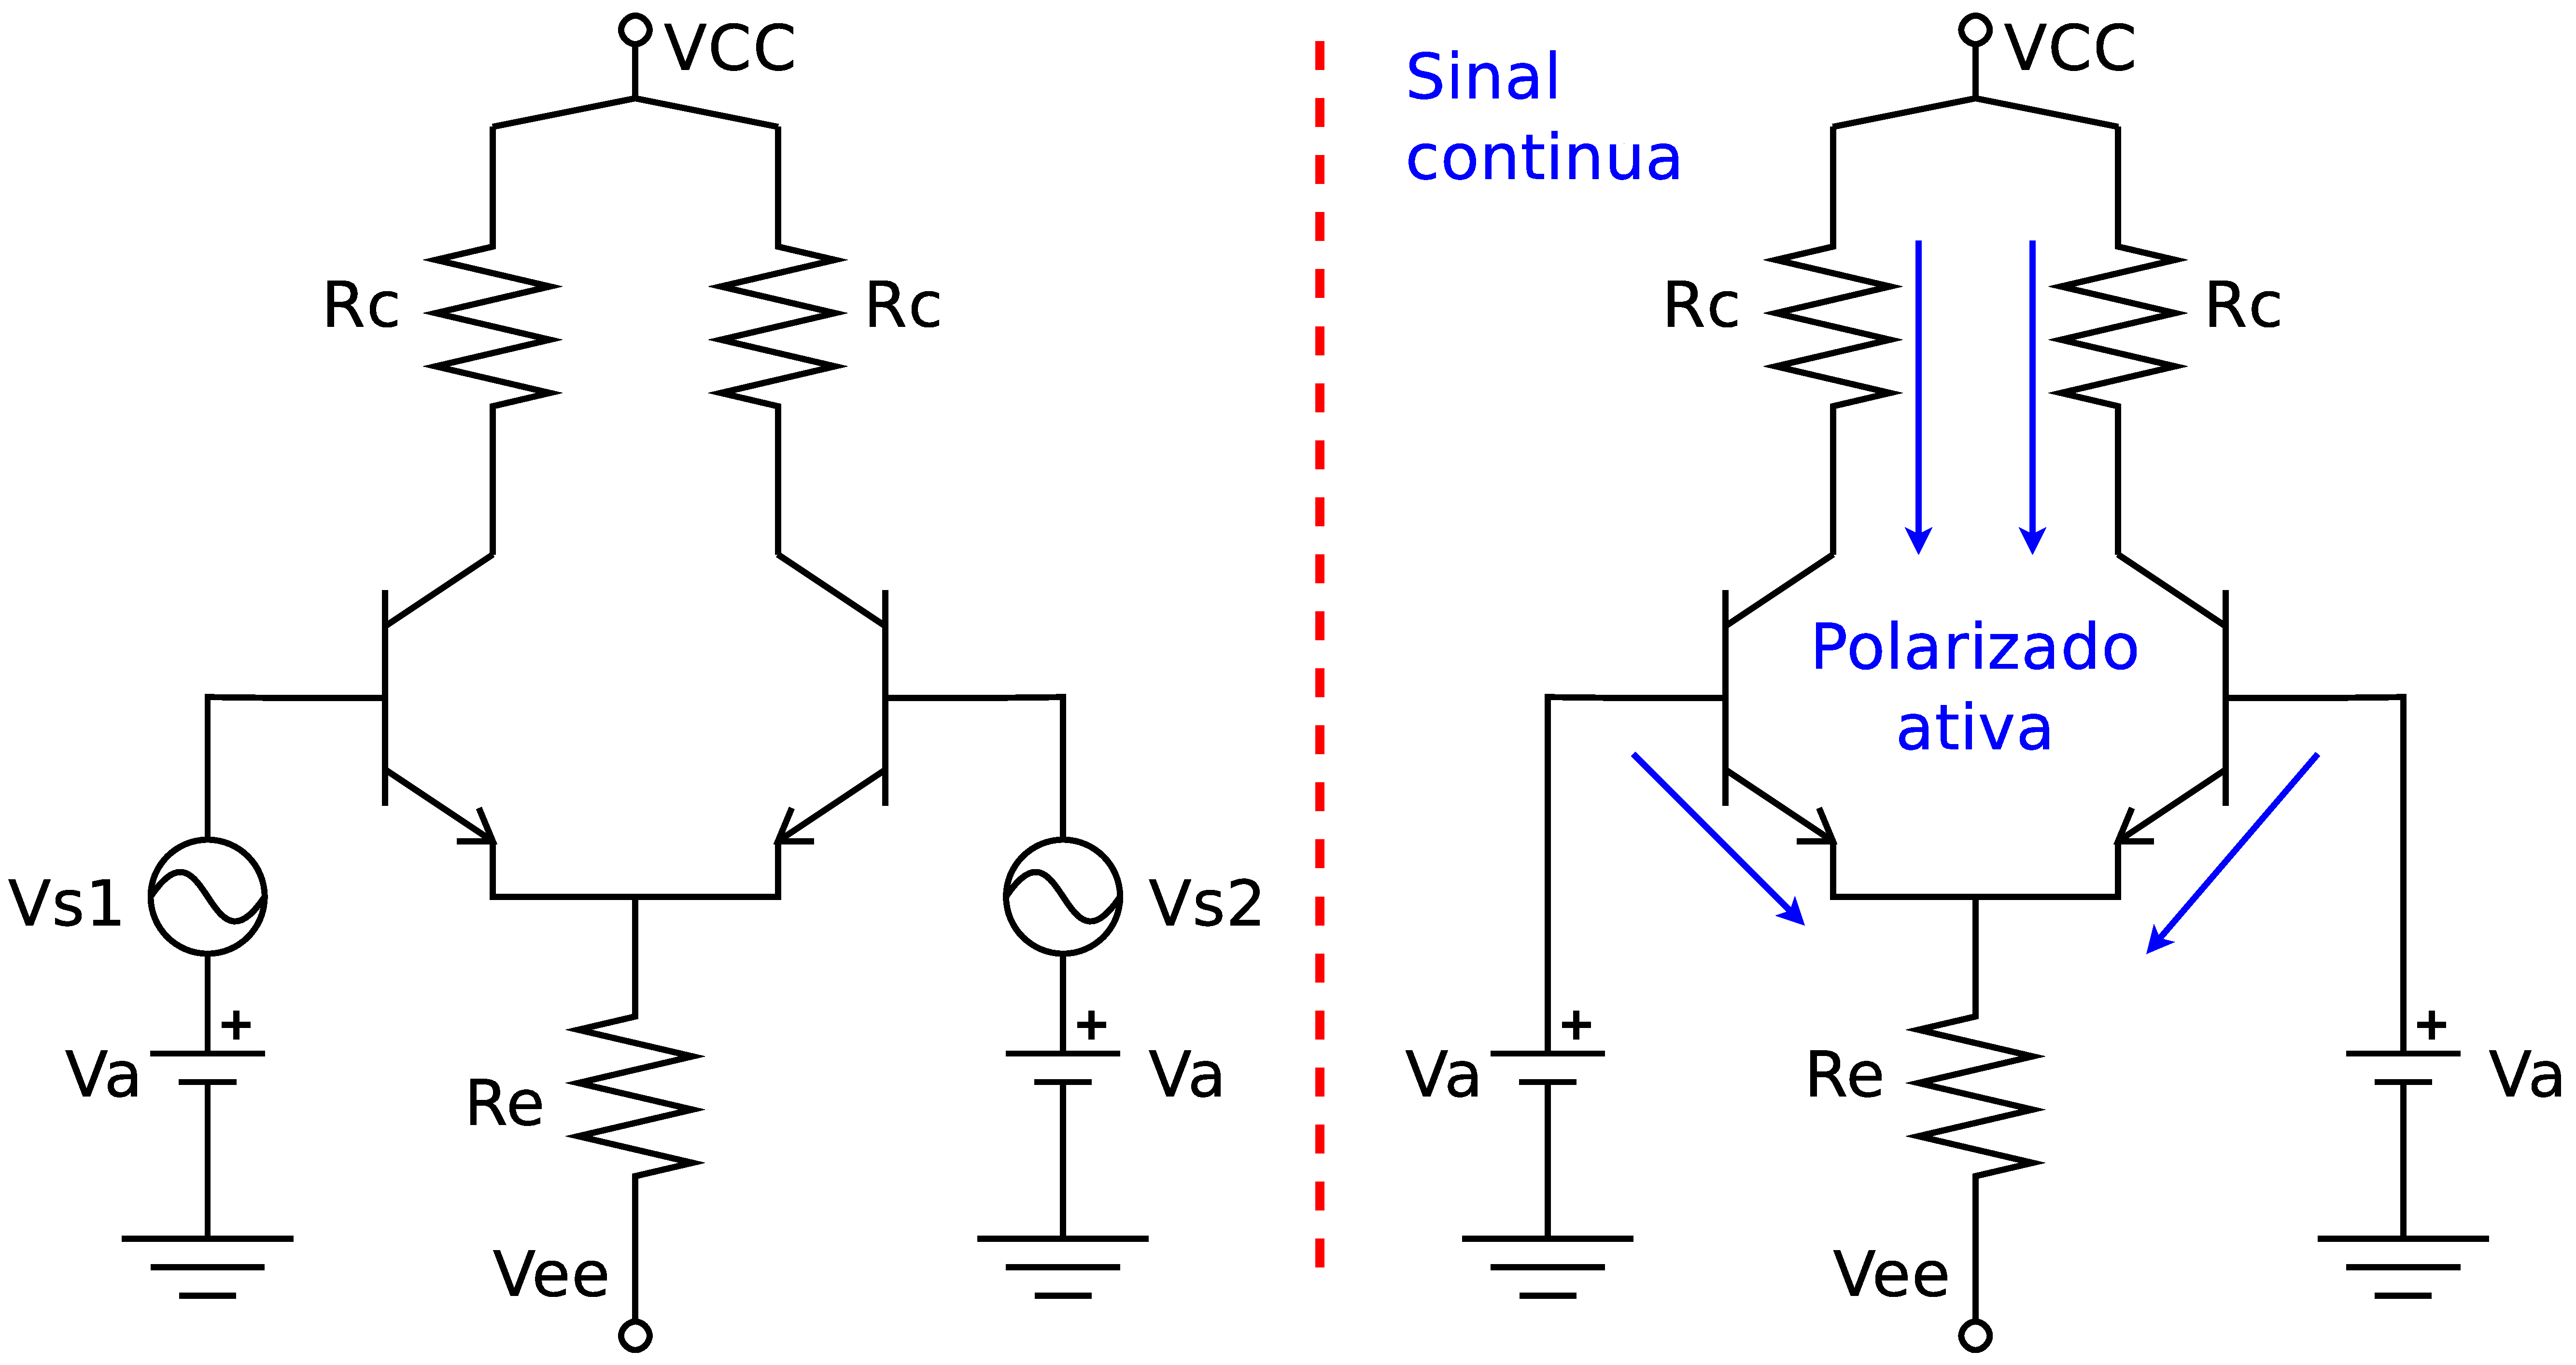
\includegraphics[width=0.99\textwidth]{images/diferencial.eps}
\end{center} 
\end{frame}
\begin{frame}{Amplificador Diferencial}
Amplificador Diferencial transistorizado
\begin{center}
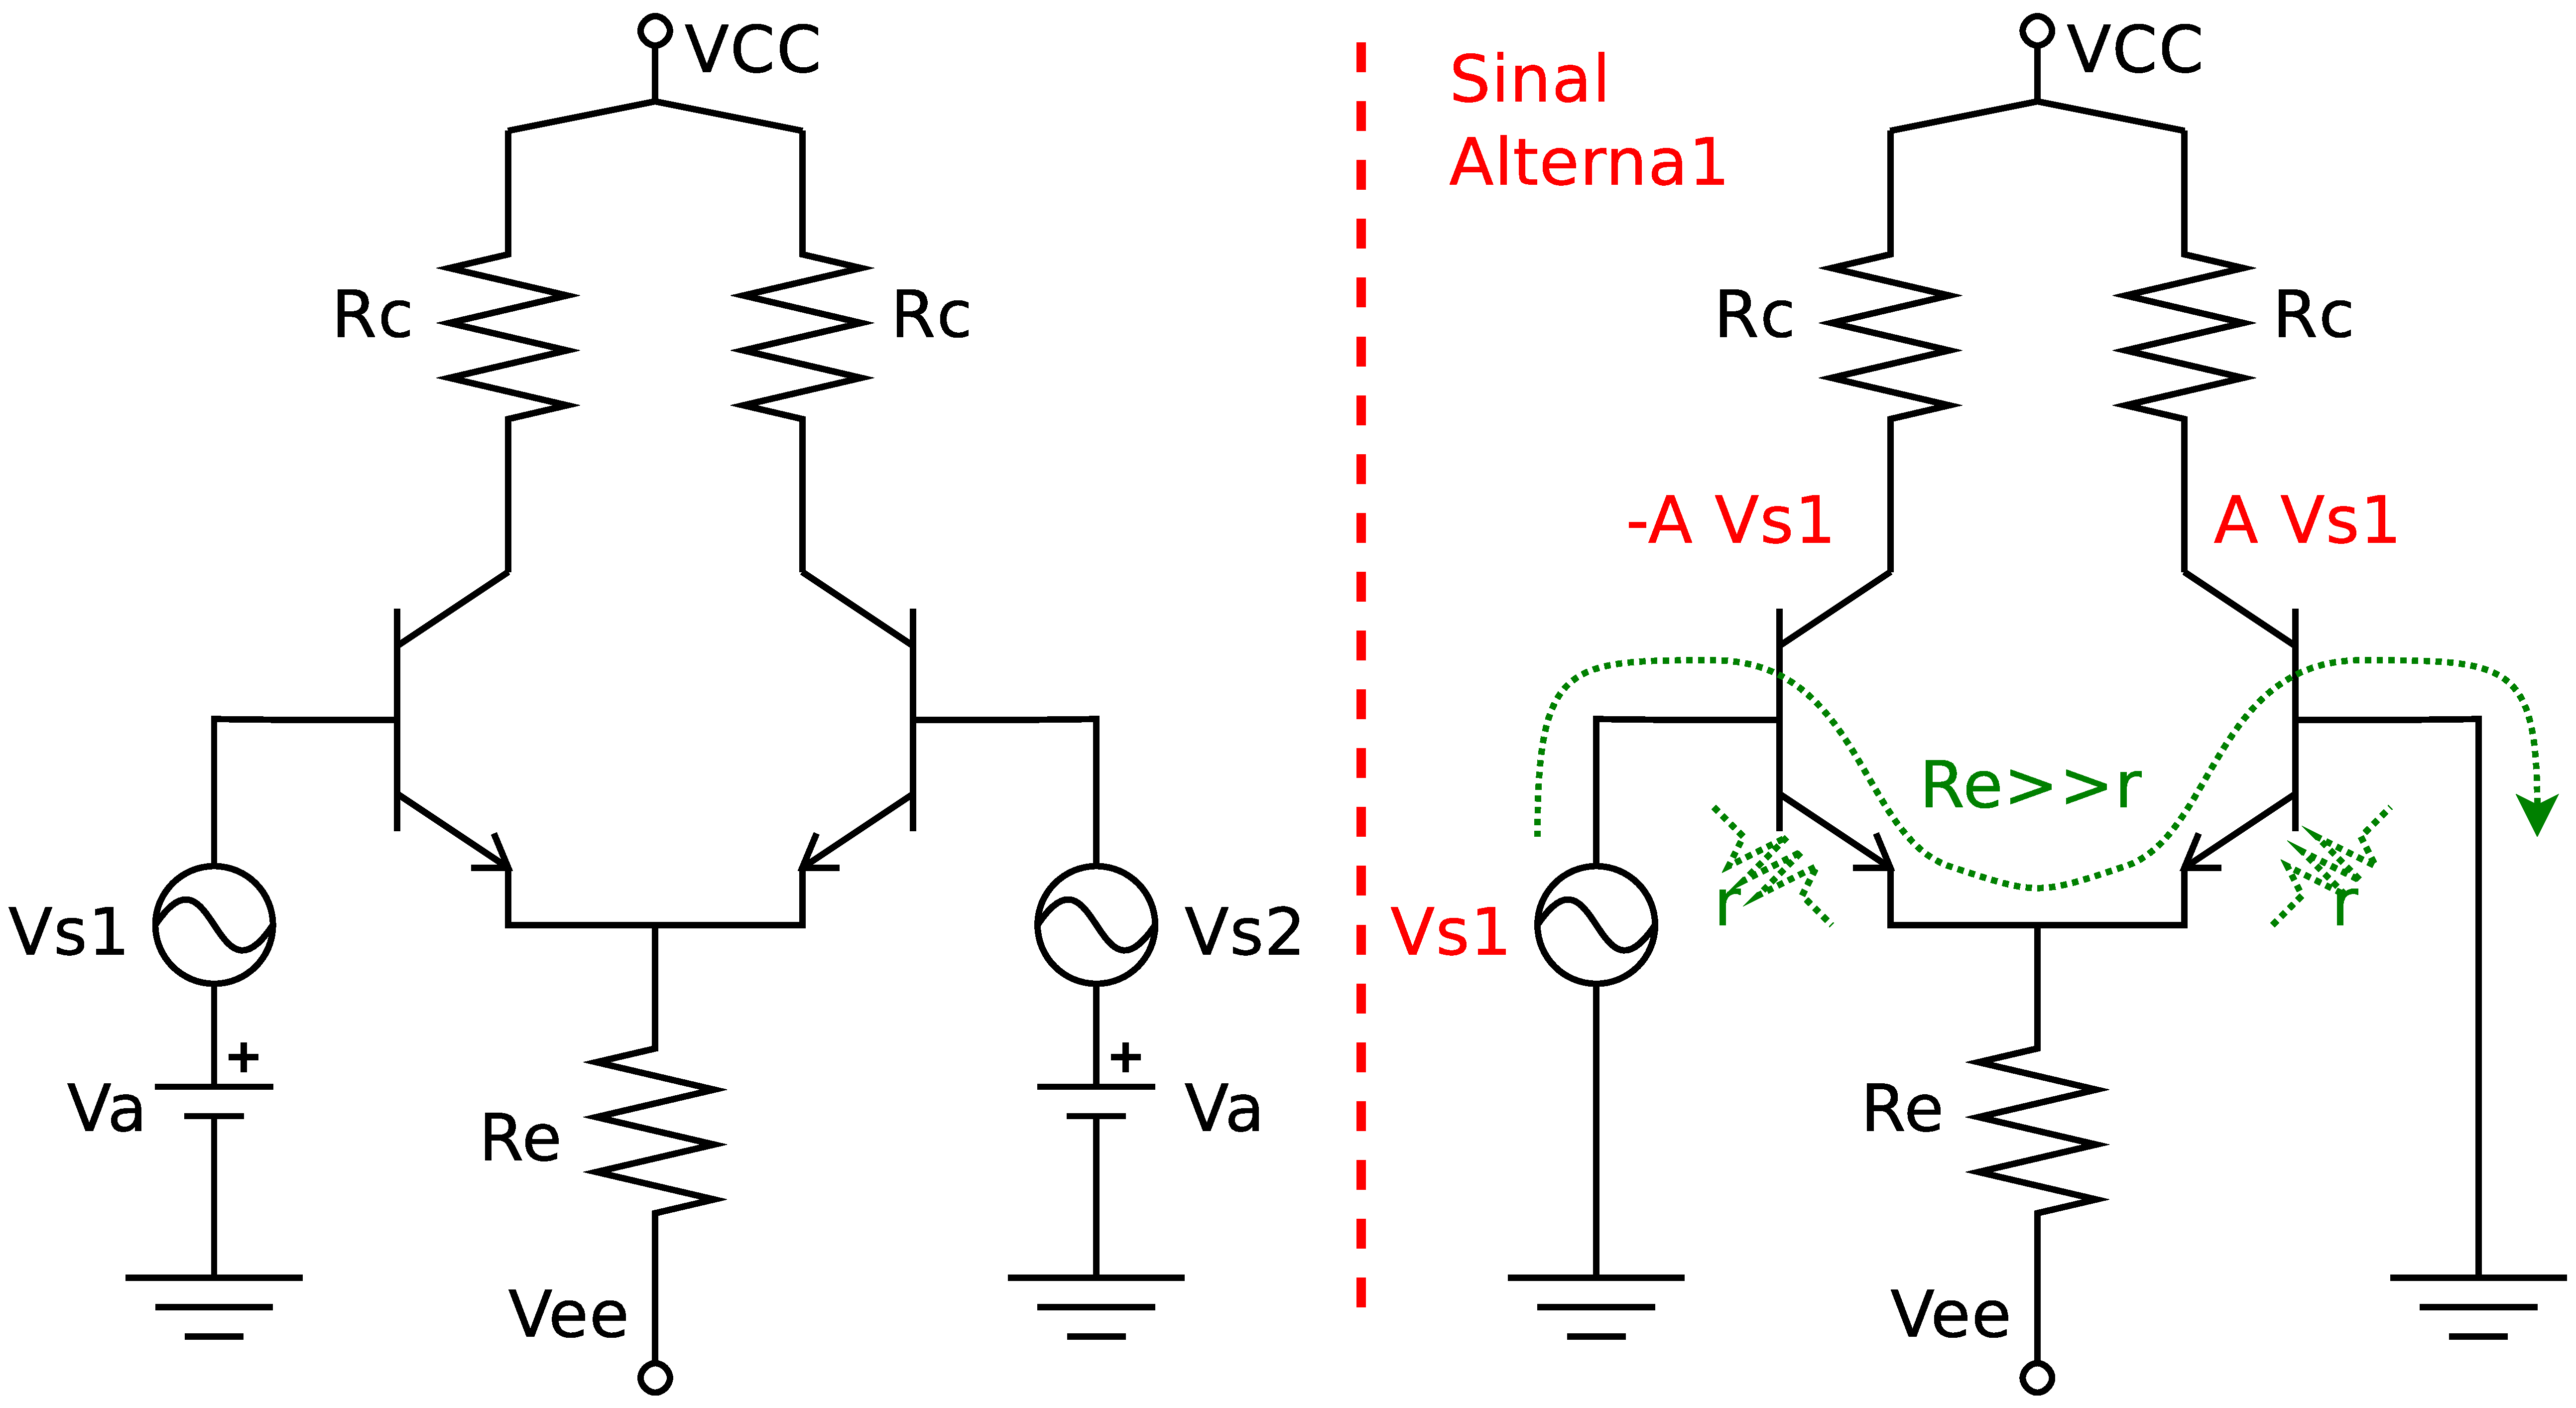
\includegraphics[width=0.99\textwidth]{images/diferencial2.eps}
\end{center} 
\end{frame}
\begin{frame}{Amplificador Diferencial}
Amplificador Diferencial transistorizado
\begin{center}
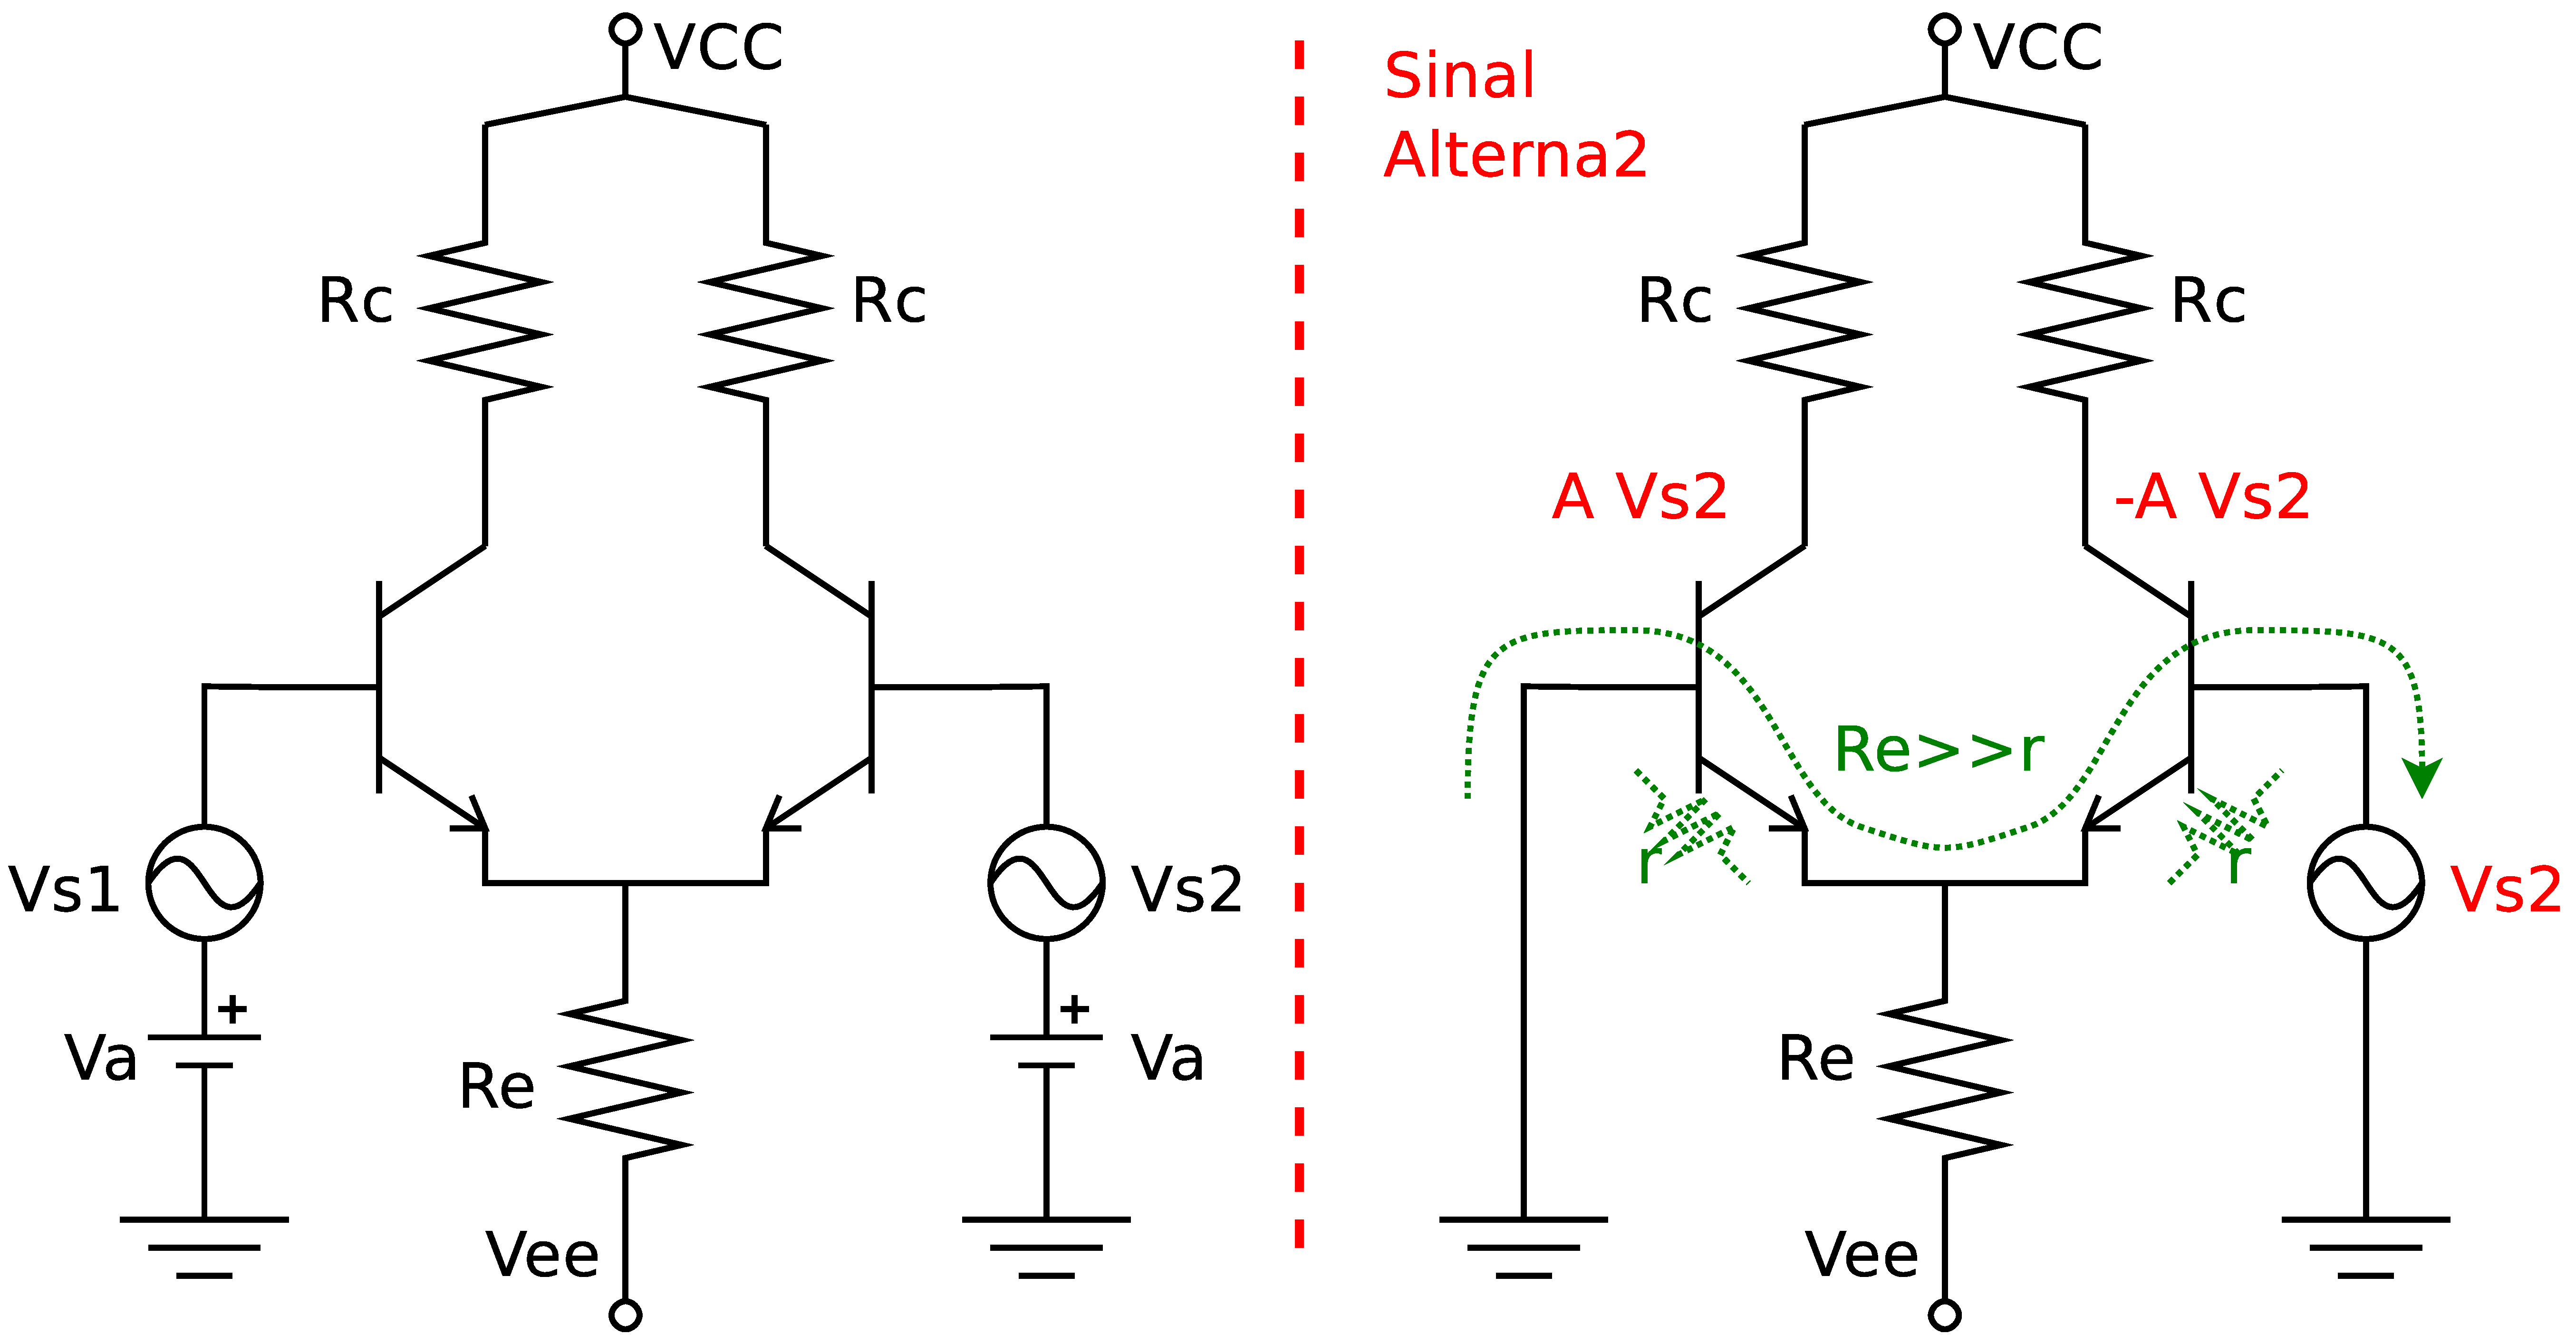
\includegraphics[width=0.99\textwidth]{images/diferencial3.eps}
\end{center} 
\end{frame}
\begin{frame}{Amplificador Diferencial}
\begin{minipage}[c]{0.5\textwidth}
\begin{center}
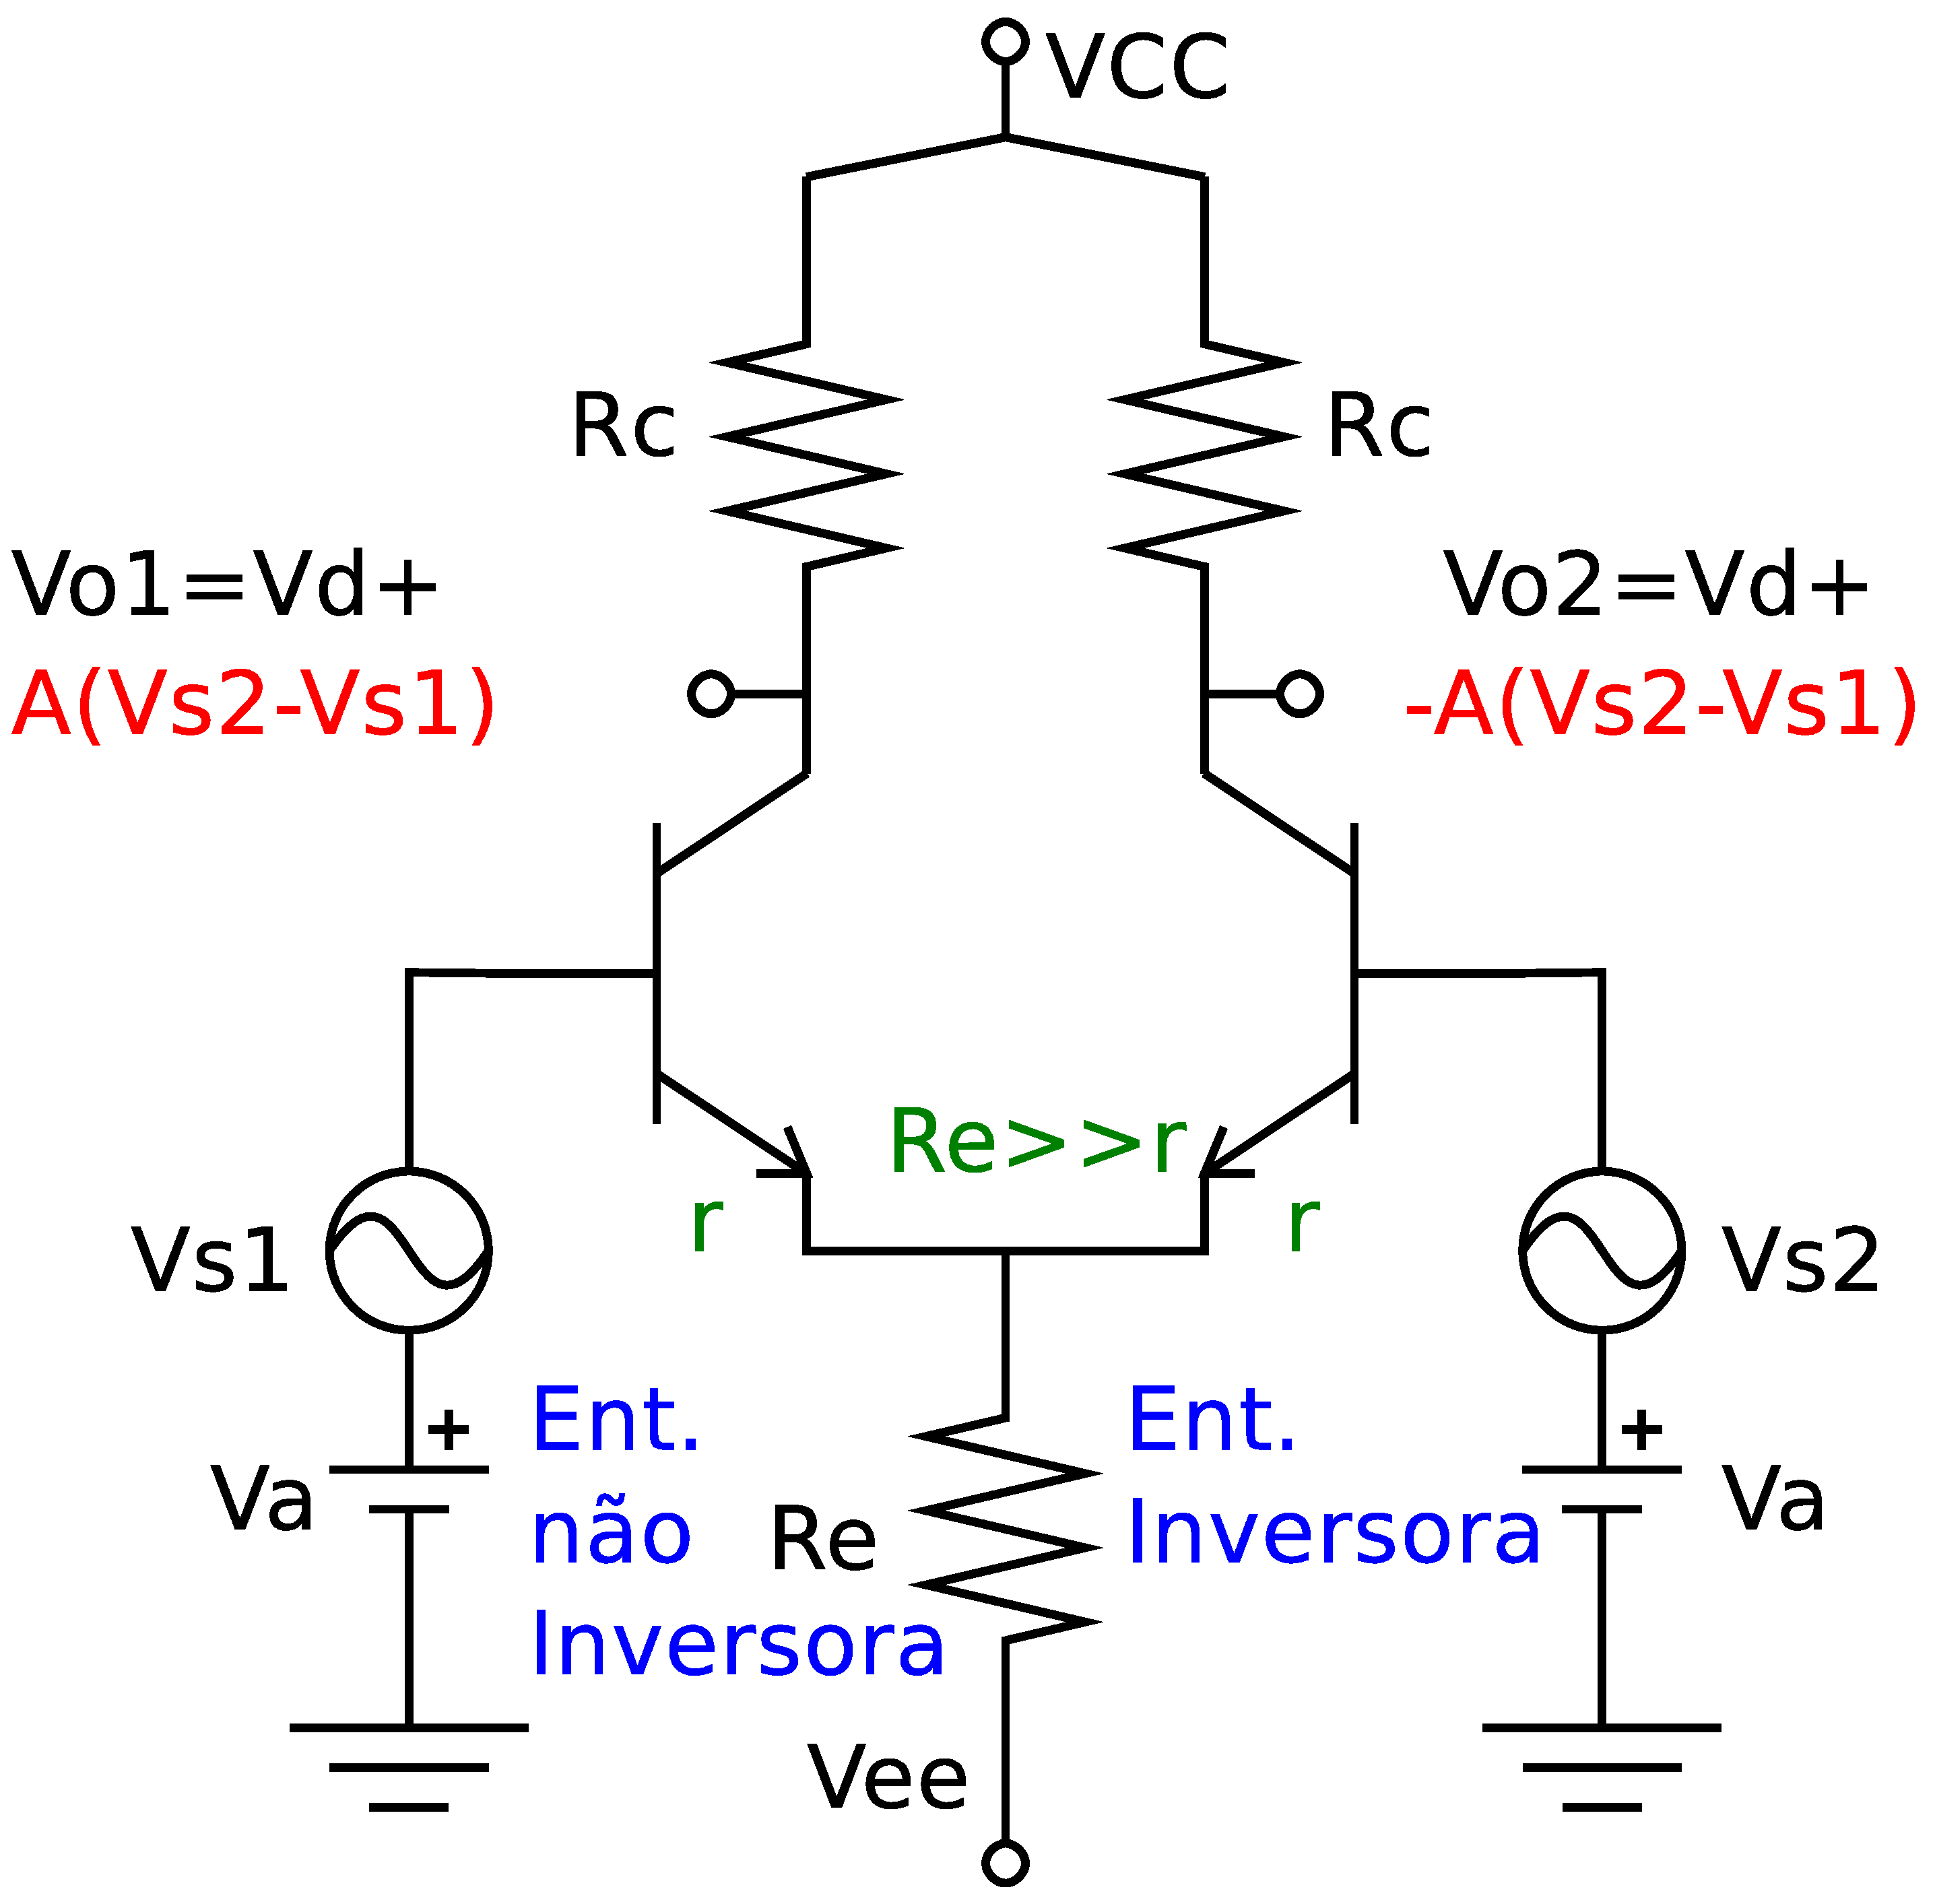
\includegraphics[width=0.99\textwidth]{images/diferencial4.eps}
\end{center}  
\end{minipage}%
\begin{minipage}[c]{0.5\textwidth}
 \begin{equation*}
  \begin{matrix}
  V_{out} & = & V_{o2}-V_{o1}   \\
  ~ & = & 2 A (V_{s1}-V_{s2})
  \end{matrix}
 \end{equation*}
\end{minipage}



\end{frame}

%%%%%%%%%%%%%%%%%%%%%%%%%%%%%%%%%%%%%%%%%%%%%%%%%%%%%%%%%%%%%%%%%%%%%%%%%%%%%%%%
\begin{frame}{Opamp Ideal}
Amplificador Operacional = OpAmp
\begin{center}
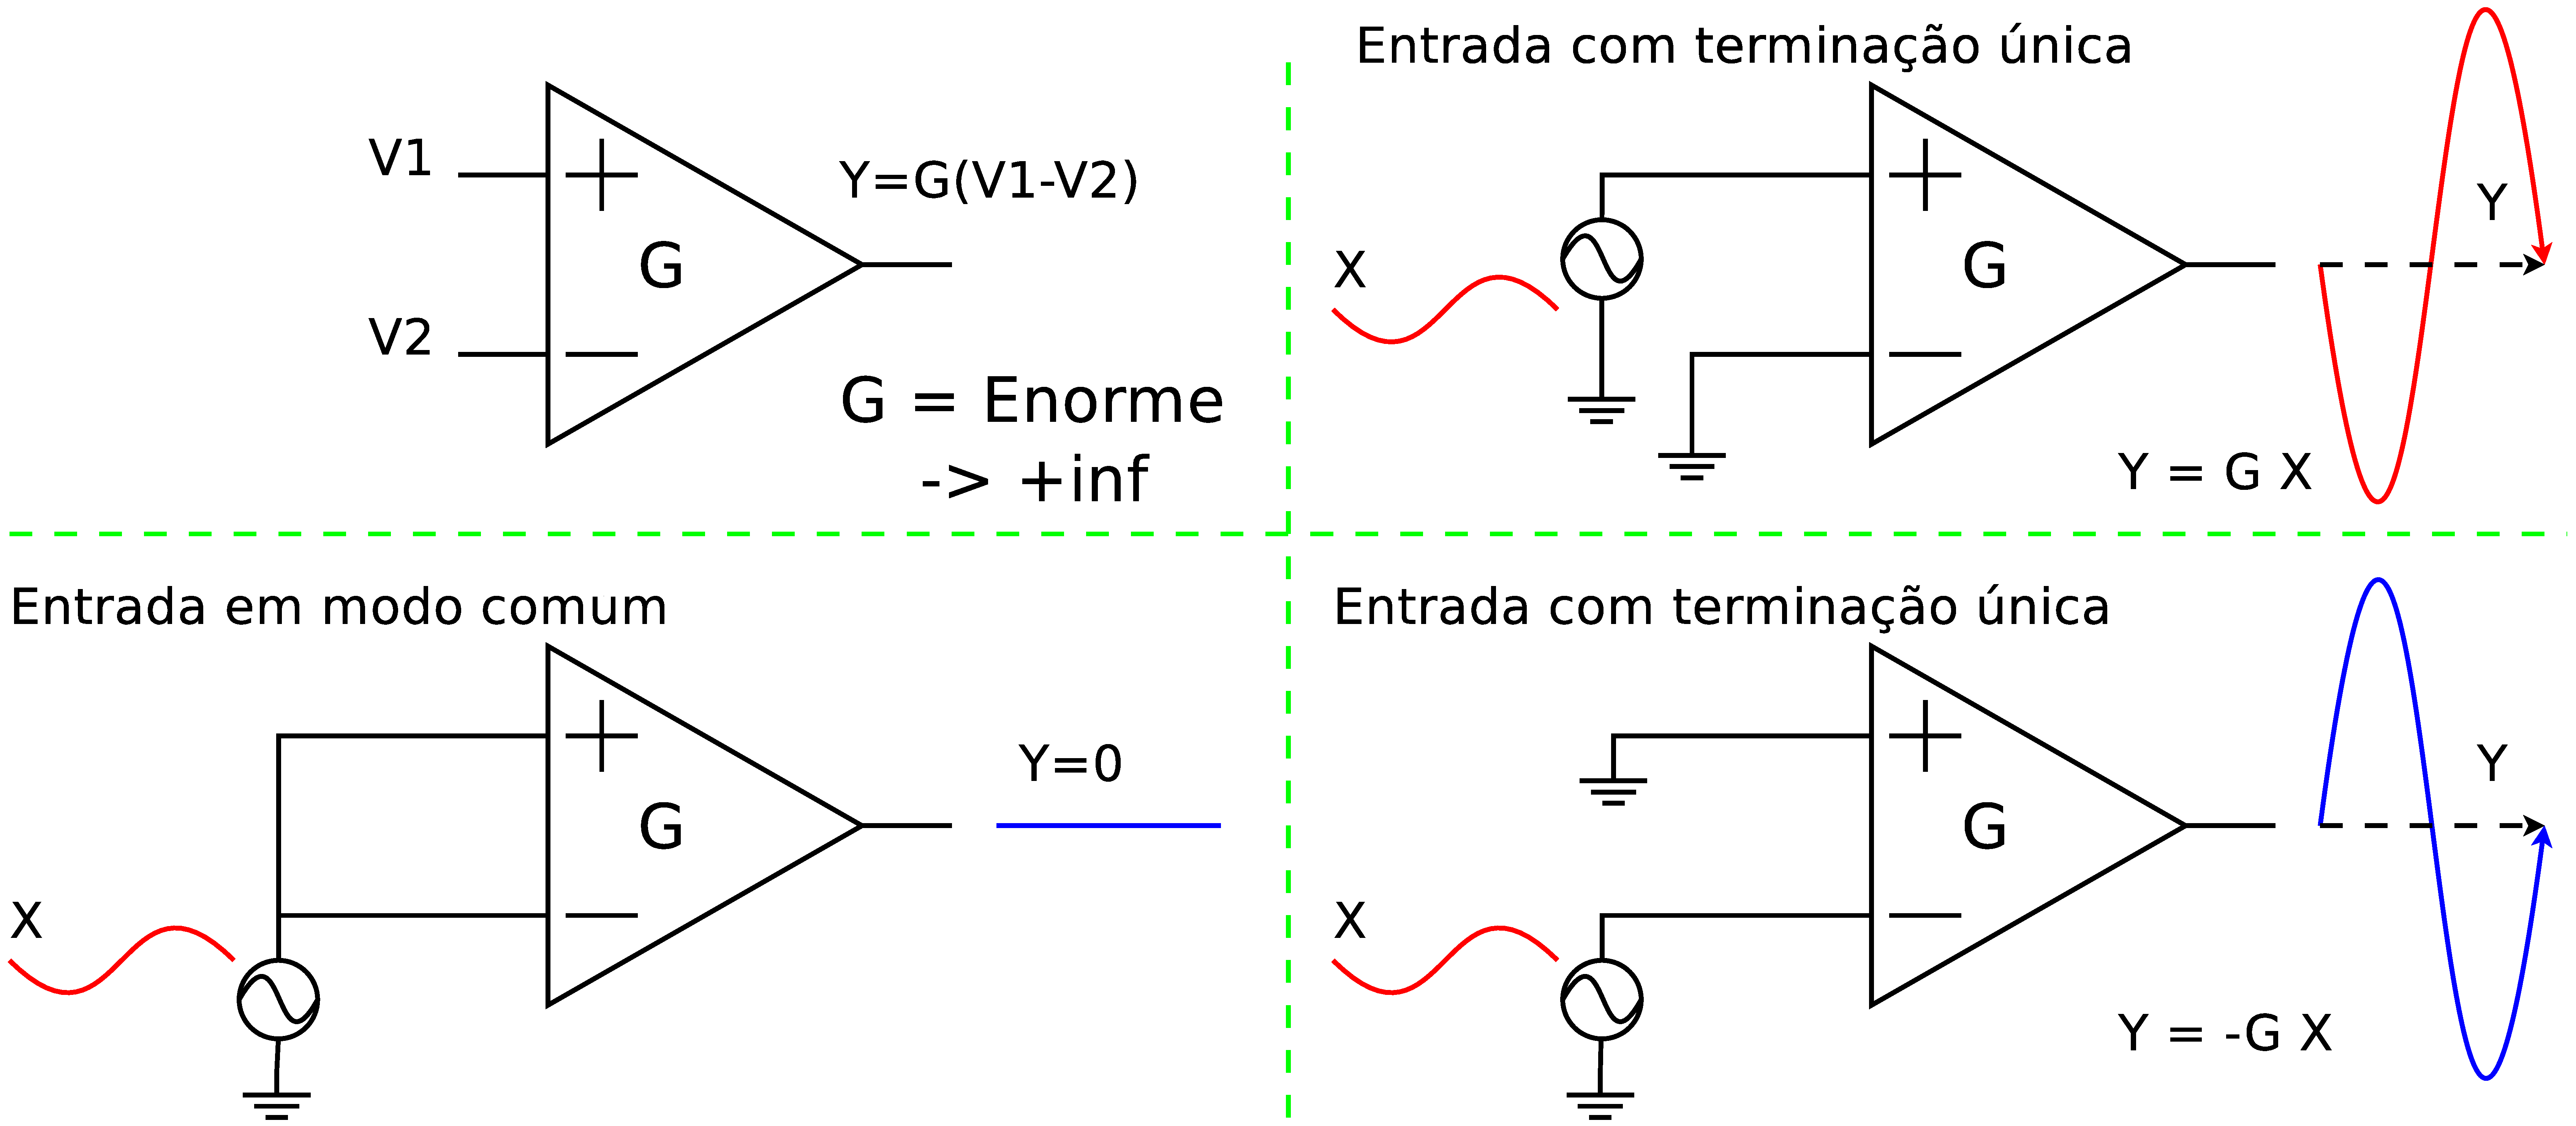
\includegraphics[width=0.99\textwidth]{images/Opamp1.eps}
\end{center} 
\end{frame}

%%%%%%%%%%%%%%%%%%%%%%%%%%%%%%%%%%%%%%%%%%%%%%%%%%%%%%%%%%%%%%%%%%%%%%%%%%%%%%%%
\begin{frame}{Opamp Ideal considerando CMRR}
\begin{center}
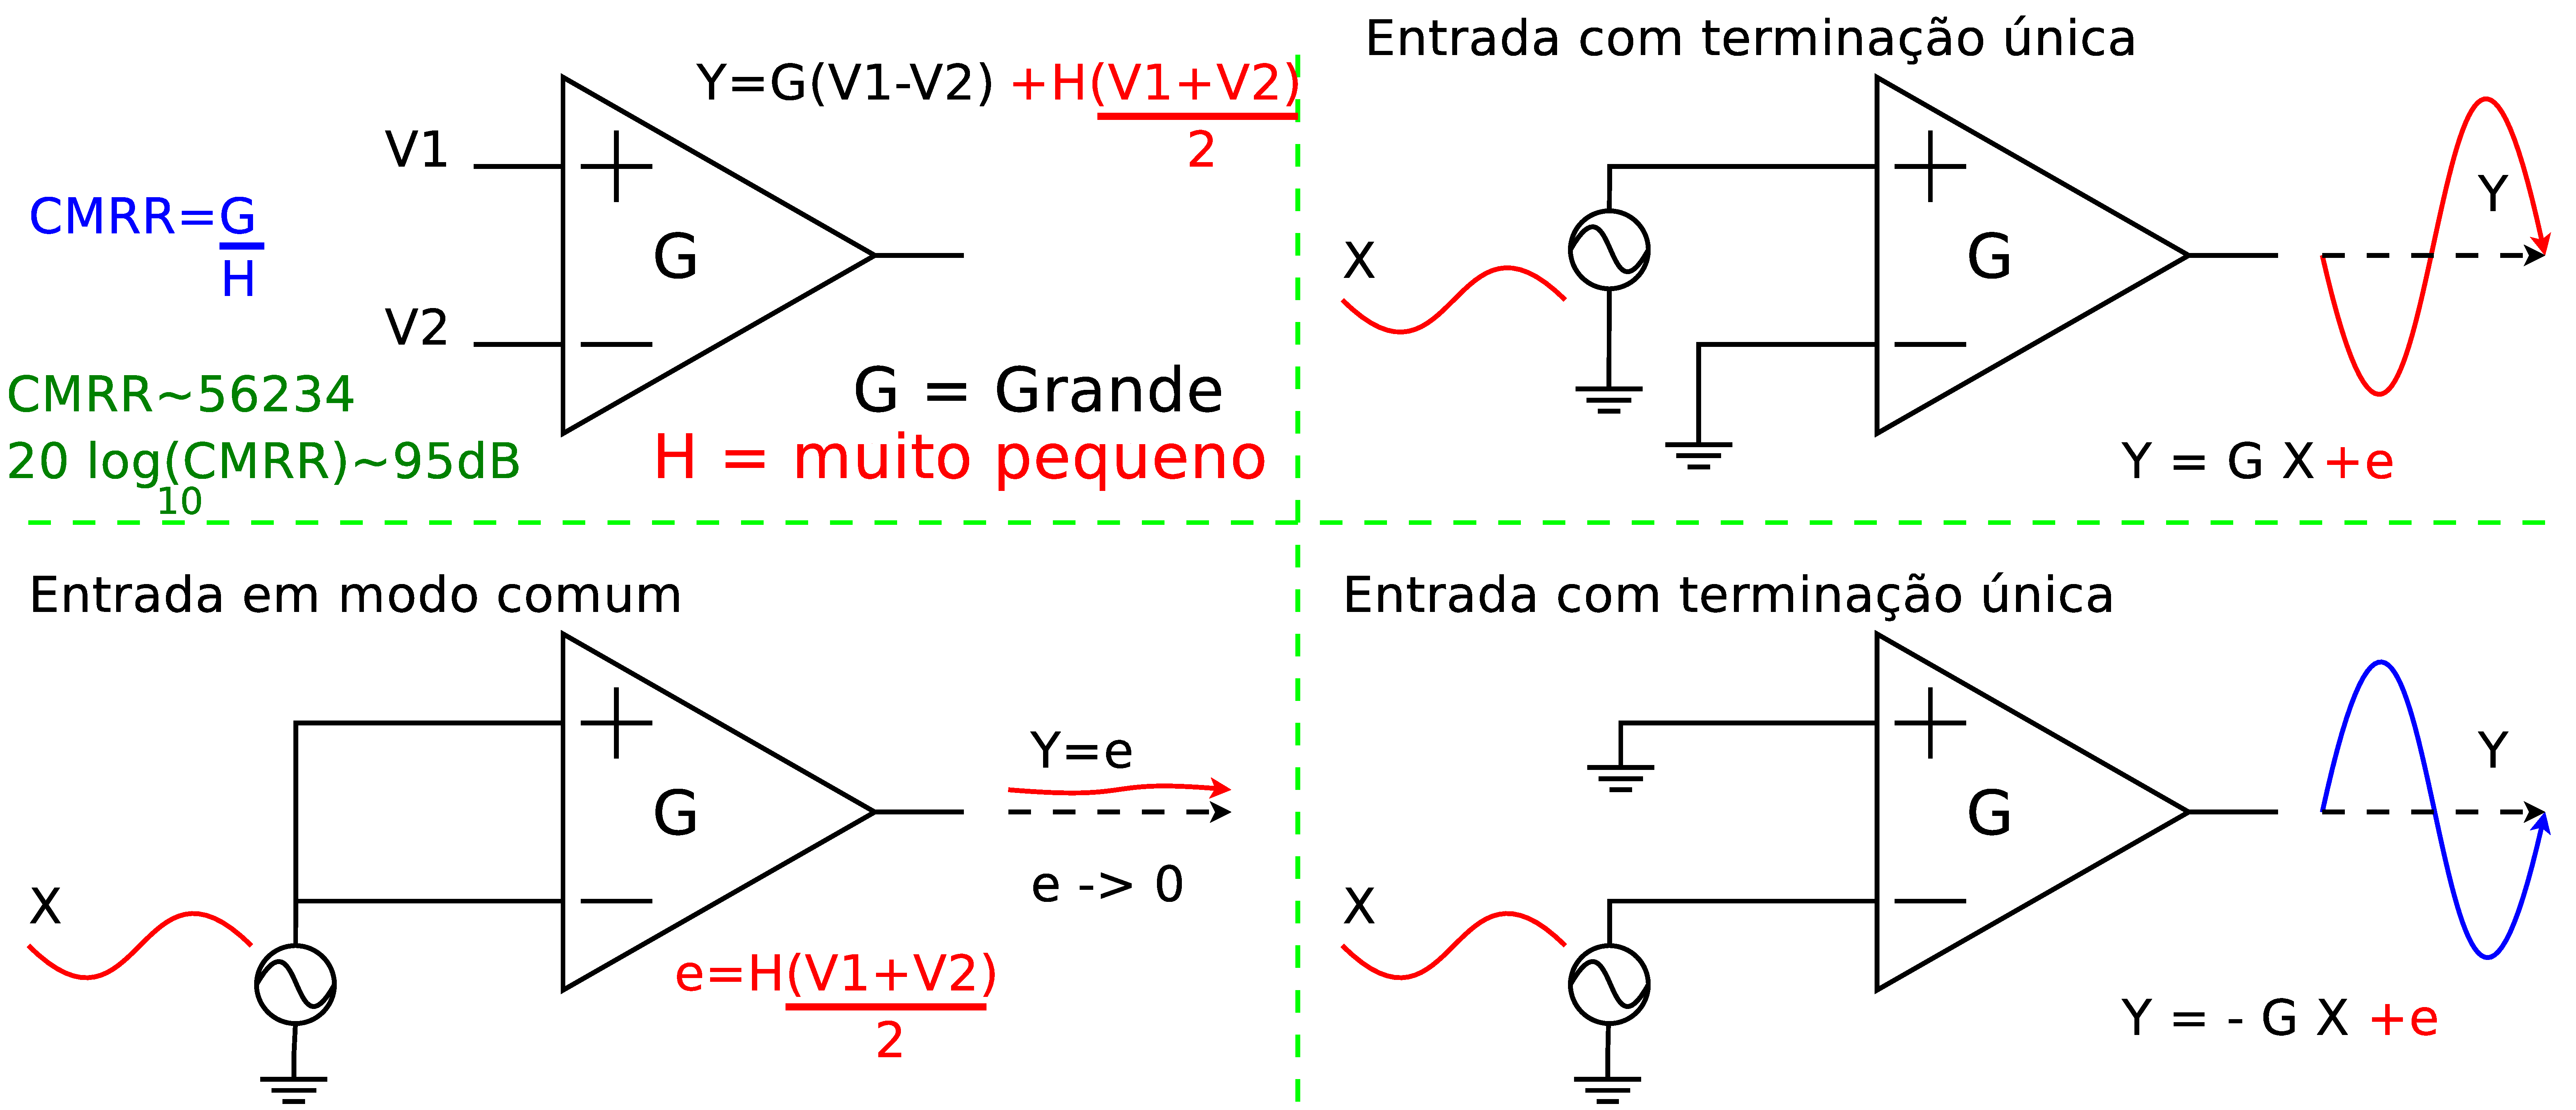
\includegraphics[width=0.99\textwidth]{images/Opamp2.eps}
\end{center} 
\end{frame}

%%%%%%%%%%%%%%%%%%%%%%%%%%%%%%%%%%%%%%%%%%%%%%%%%%%%%%%%%%%%%%%%%%%%%%%%%%%%%%%%
\begin{frame}{Opamp prático}
\begin{center}
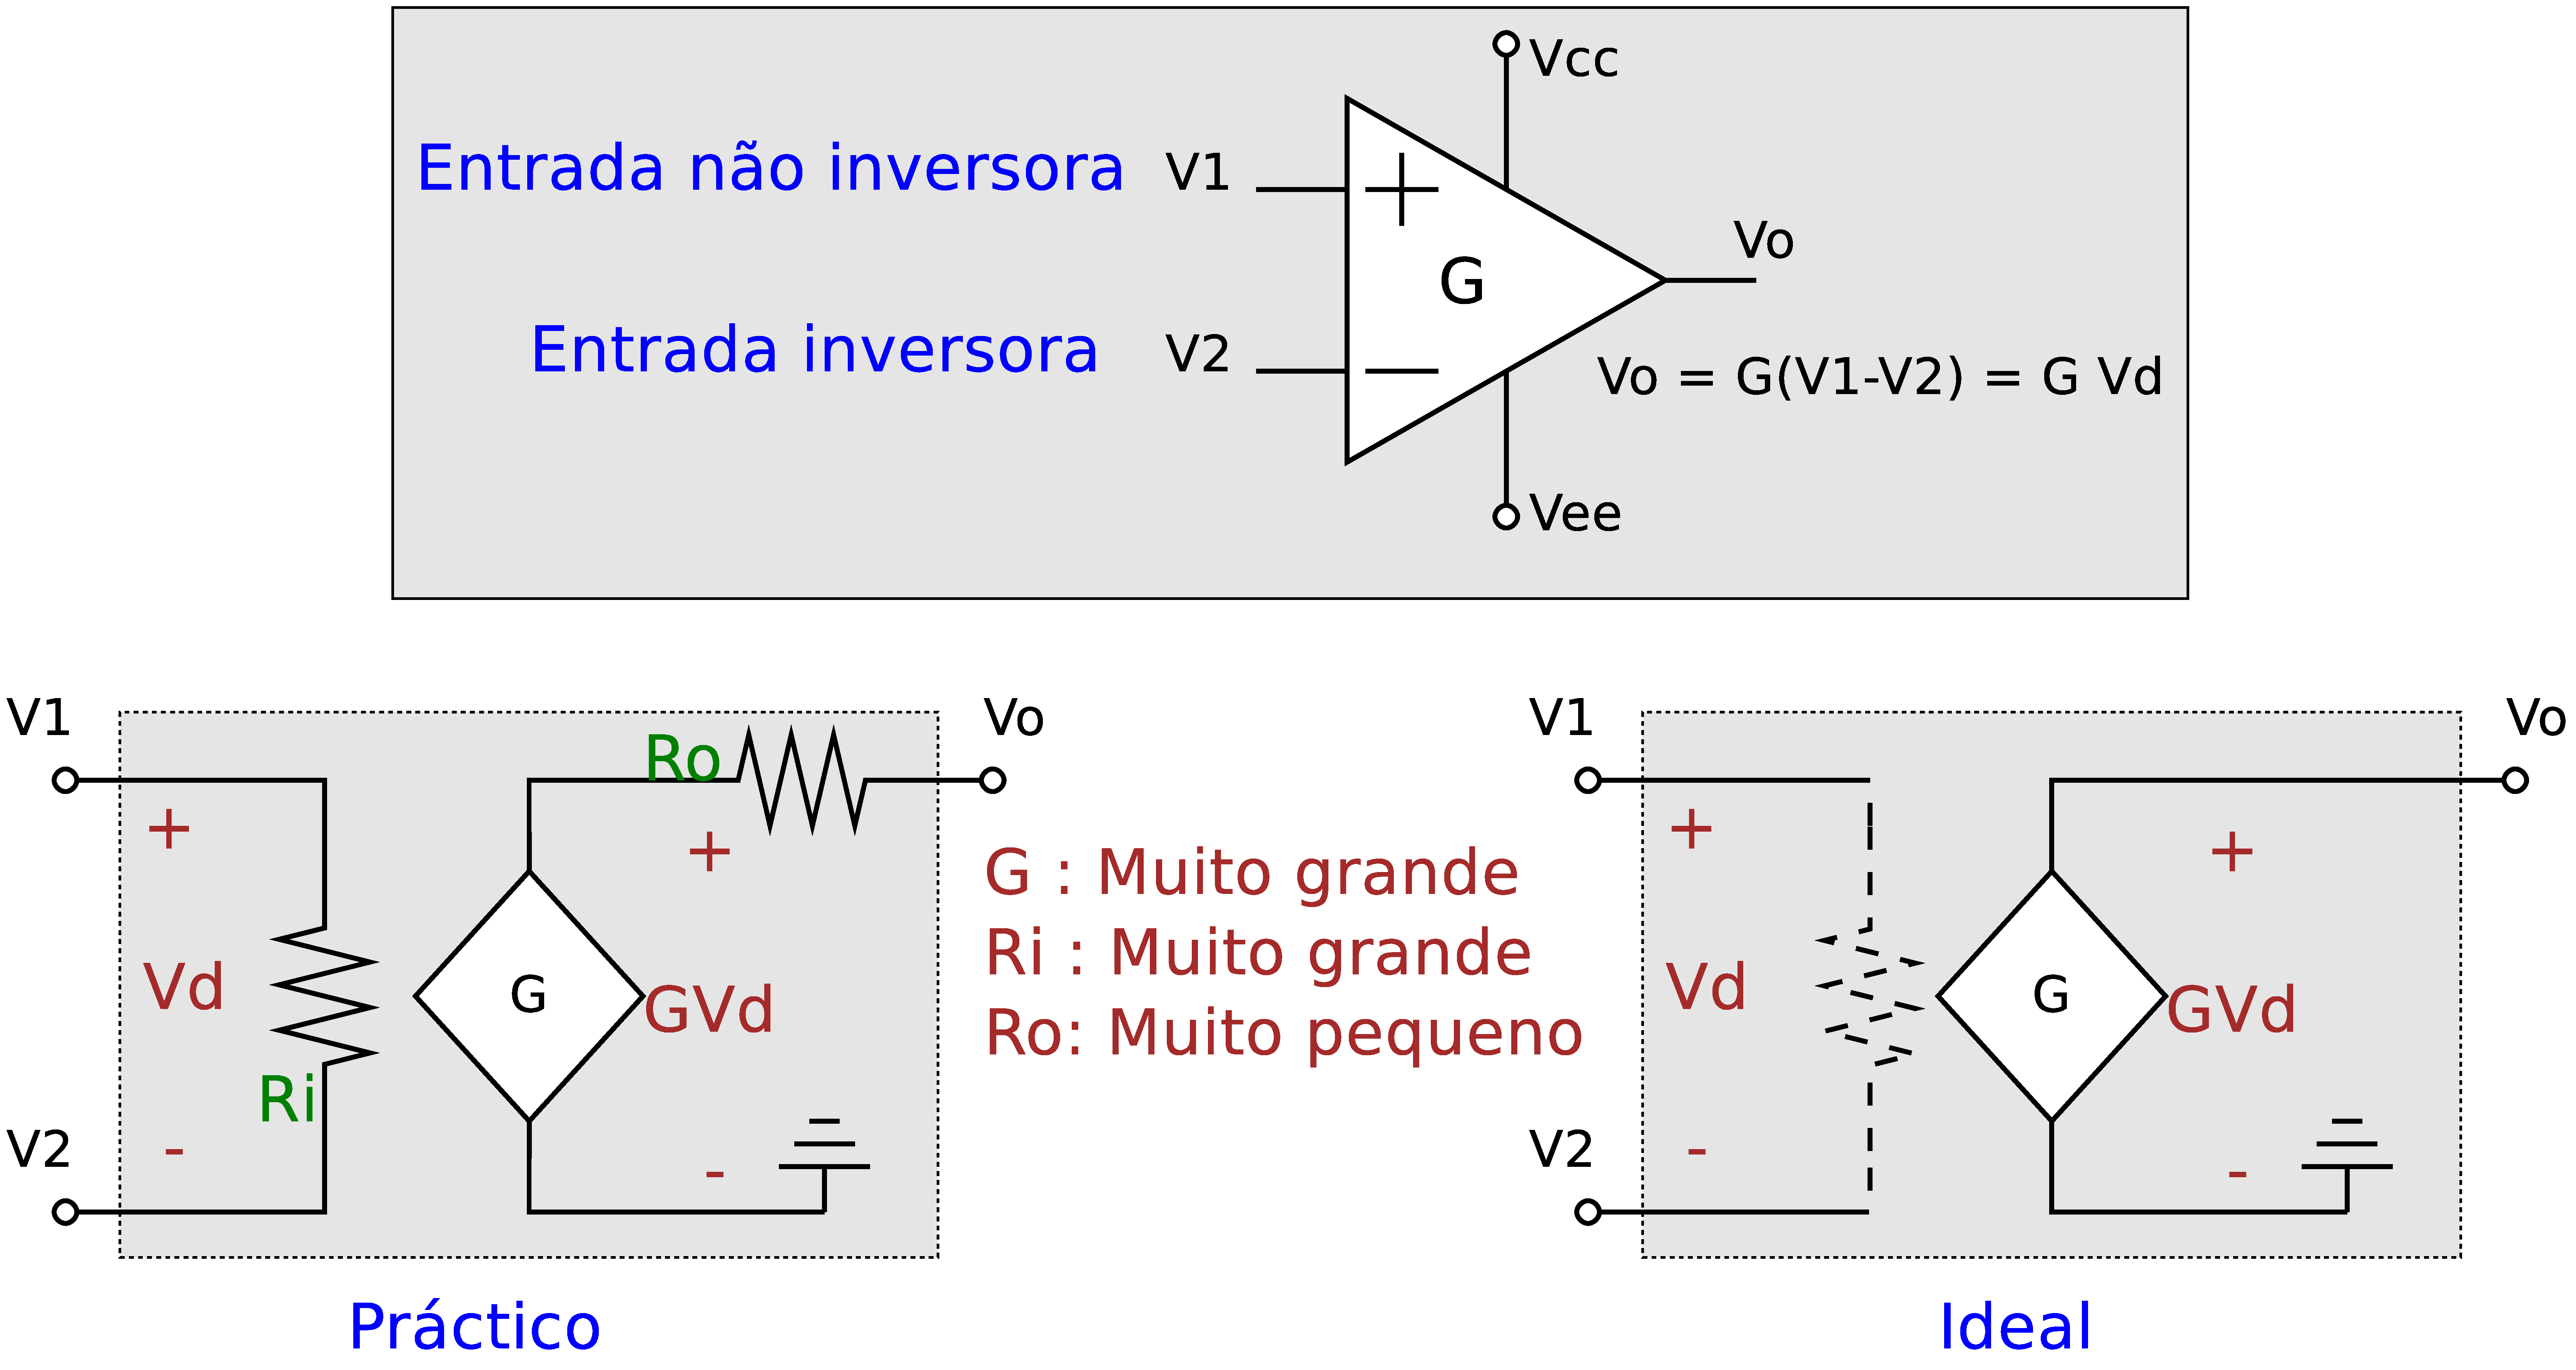
\includegraphics[width=0.99\textwidth]{images/Opamp3.eps}
\end{center} 
\end{frame}


%%%%%%%%%%%%%%%%%%%%%%%%%%%%%%%%%%%%%%%%%%%%%%%%%%%%%%%%%%%%%%%%%%%%%%%%%%%%%%%%
\begin{frame}{Opamp ideal}
\begin{center}
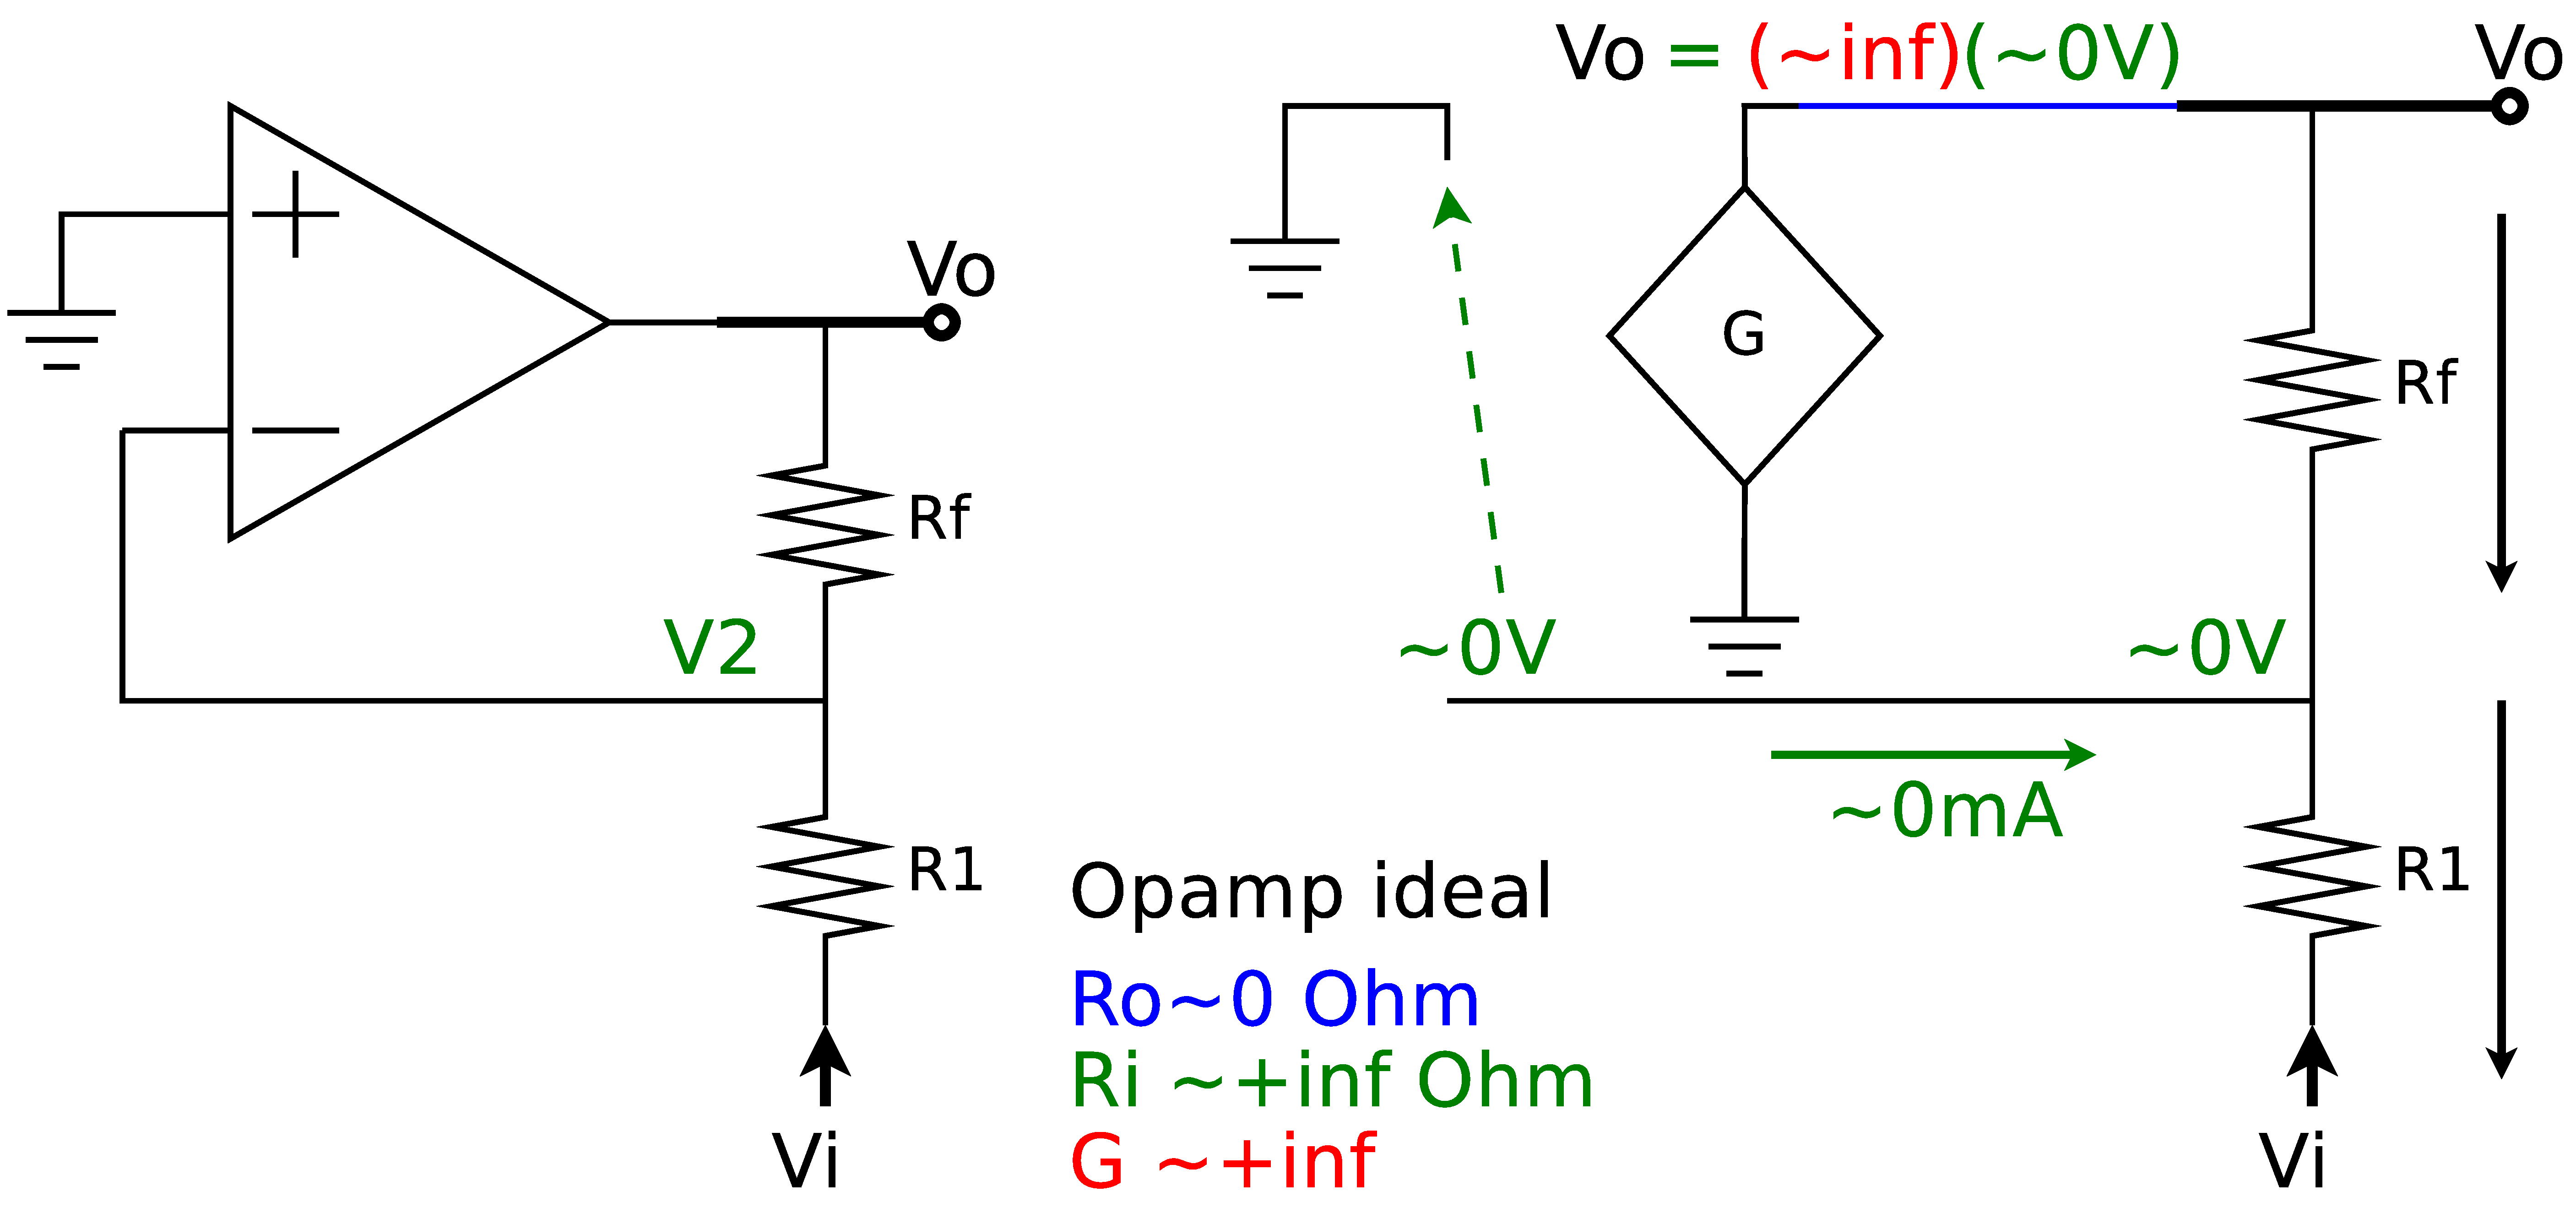
\includegraphics[width=0.8\textwidth]{images/Ejemplo1ideal.eps}
\begin{equation*}
 \frac{V_o}{R_f}=\frac{-V_i}{R_1} ~~~ \rightarrow ~~~ V_o=-V_i \frac{R_f}{R_1} 
\end{equation*}
\end{center} 
\end{frame}

%%%%%%%%%%%%%%%%%%%%%%%%%%%%%%%%%%%%%%%%%%%%%%%%%%%%%%%%%%%%%%%%%%%%%%%%%%%%%%%%
\begin{frame}{Opamp prático}
\begin{center}
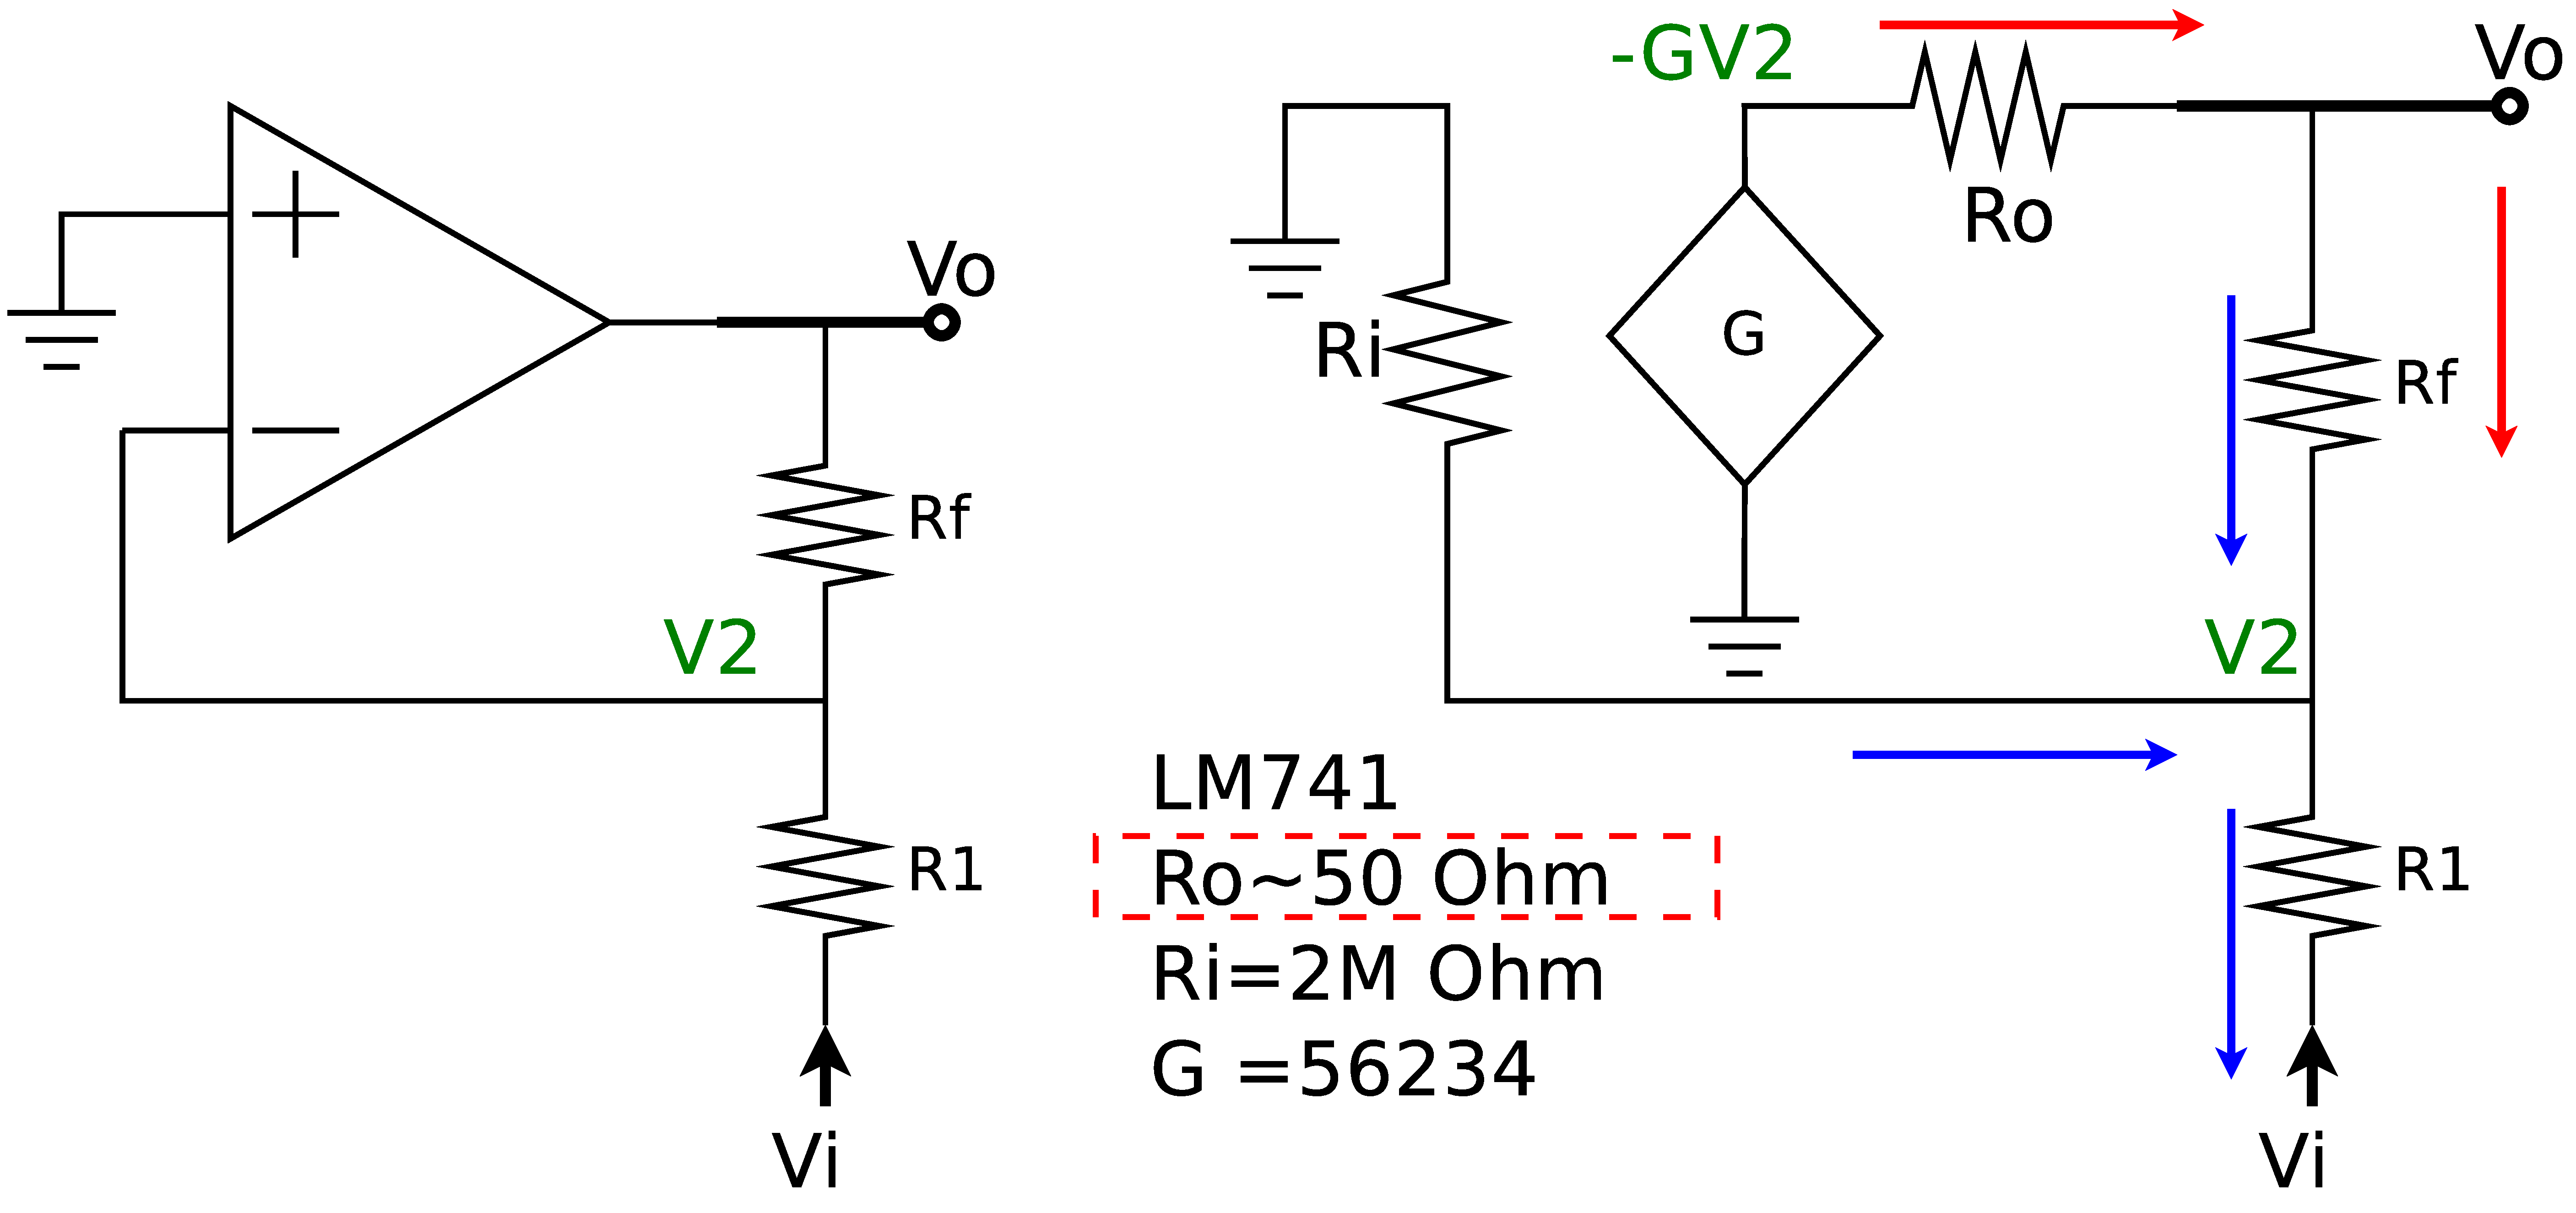
\includegraphics[width=0.8\textwidth]{images/Ejemplo1.eps}

{\color{blue} $-\frac{V_2}{R_i}+\frac{V_0-V_2}{R_f}=\frac{V_2-V_i}{R_1}$} ~~~~~~~
{\color{red} $\frac{-GV_2-V_o}{R_o}=\frac{V_o-V_2}{R_f}$}

$V_o\left( 1+R_f\frac{\left(\frac{1}{R_1}+\frac{1}{R_f}+\frac{1}{{\textcolor{red}{R_i}}} \right)\left(\frac{1}{R_f}+\frac{1}{{\textcolor{red}{R_o}}} \right)}{\left( \frac{{\textcolor{red}G}}{{\textcolor{red}{R_o}}}-\frac{1}{R_f}\right)} \right) = \frac{-R_f}{R_1}V_i$
\end{center} 
\end{frame}
\begin{frame}{Opamp prático}
~
{\textcolor{red}{Quando este fator tende a zero?:}}~~~
$R_f\frac{\left(\frac{1}{R_1}+\frac{1}{R_f}+\frac{1}{{\textcolor{red}{R_i}}} \right)\left(\frac{1}{R_f}+\frac{1}{{\textcolor{red}{R_o}}} \right)}{\left( \frac{{\textcolor{red}G}}{{\textcolor{red}{R_o}}}-\frac{1}{R_f}\right)}$ \\
\noindent\rule{\linewidth}{0.4pt}
Simplificando assumindo $R_f >> R_o$ :~~~
$R_f\frac{\left(\frac{1}{R_1}+\frac{1}{R_f}+\frac{1}{{\textcolor{red}{R_i}}} \right)\left(\frac{1}{{\textcolor{red}{R_o}}} \right)}{\left( \frac{{\textcolor{red}G}}{{\textcolor{red}{R_o}}}\right)}$ 
Consequência : ~~~
$\frac{R_f}{{\textcolor{red}G} } \left(\frac{1}{R_1}+\frac{1}{R_f}+\frac{1}{{\textcolor{red}{R_i}}} \right) $\\ 
Simplificando assumindo $R_i >> R_f$ e $R_i >> R_1$ :~~~
$\frac{\left(\frac{R_f}{R_1}+1  \right)}{{\textcolor{red}G} }$ 
Simplificando assumindo $G >>\frac{ R_f }{ R_1}$ :~~~${\textcolor{red}{0}}$
\end{frame}


%%%%%%%%%%%%%%%%%%%%%%%%%%%%%%%%%%%%%%%%%%%%%%%%%%%%%%%%%%%%%%%%%%%%%%%%%%%%%%%%
\begin{frame}{Quando o Opamp prático tende a Opamp ideal}
\begin{minipage}[c]{0.4\textwidth}
\begin{center}
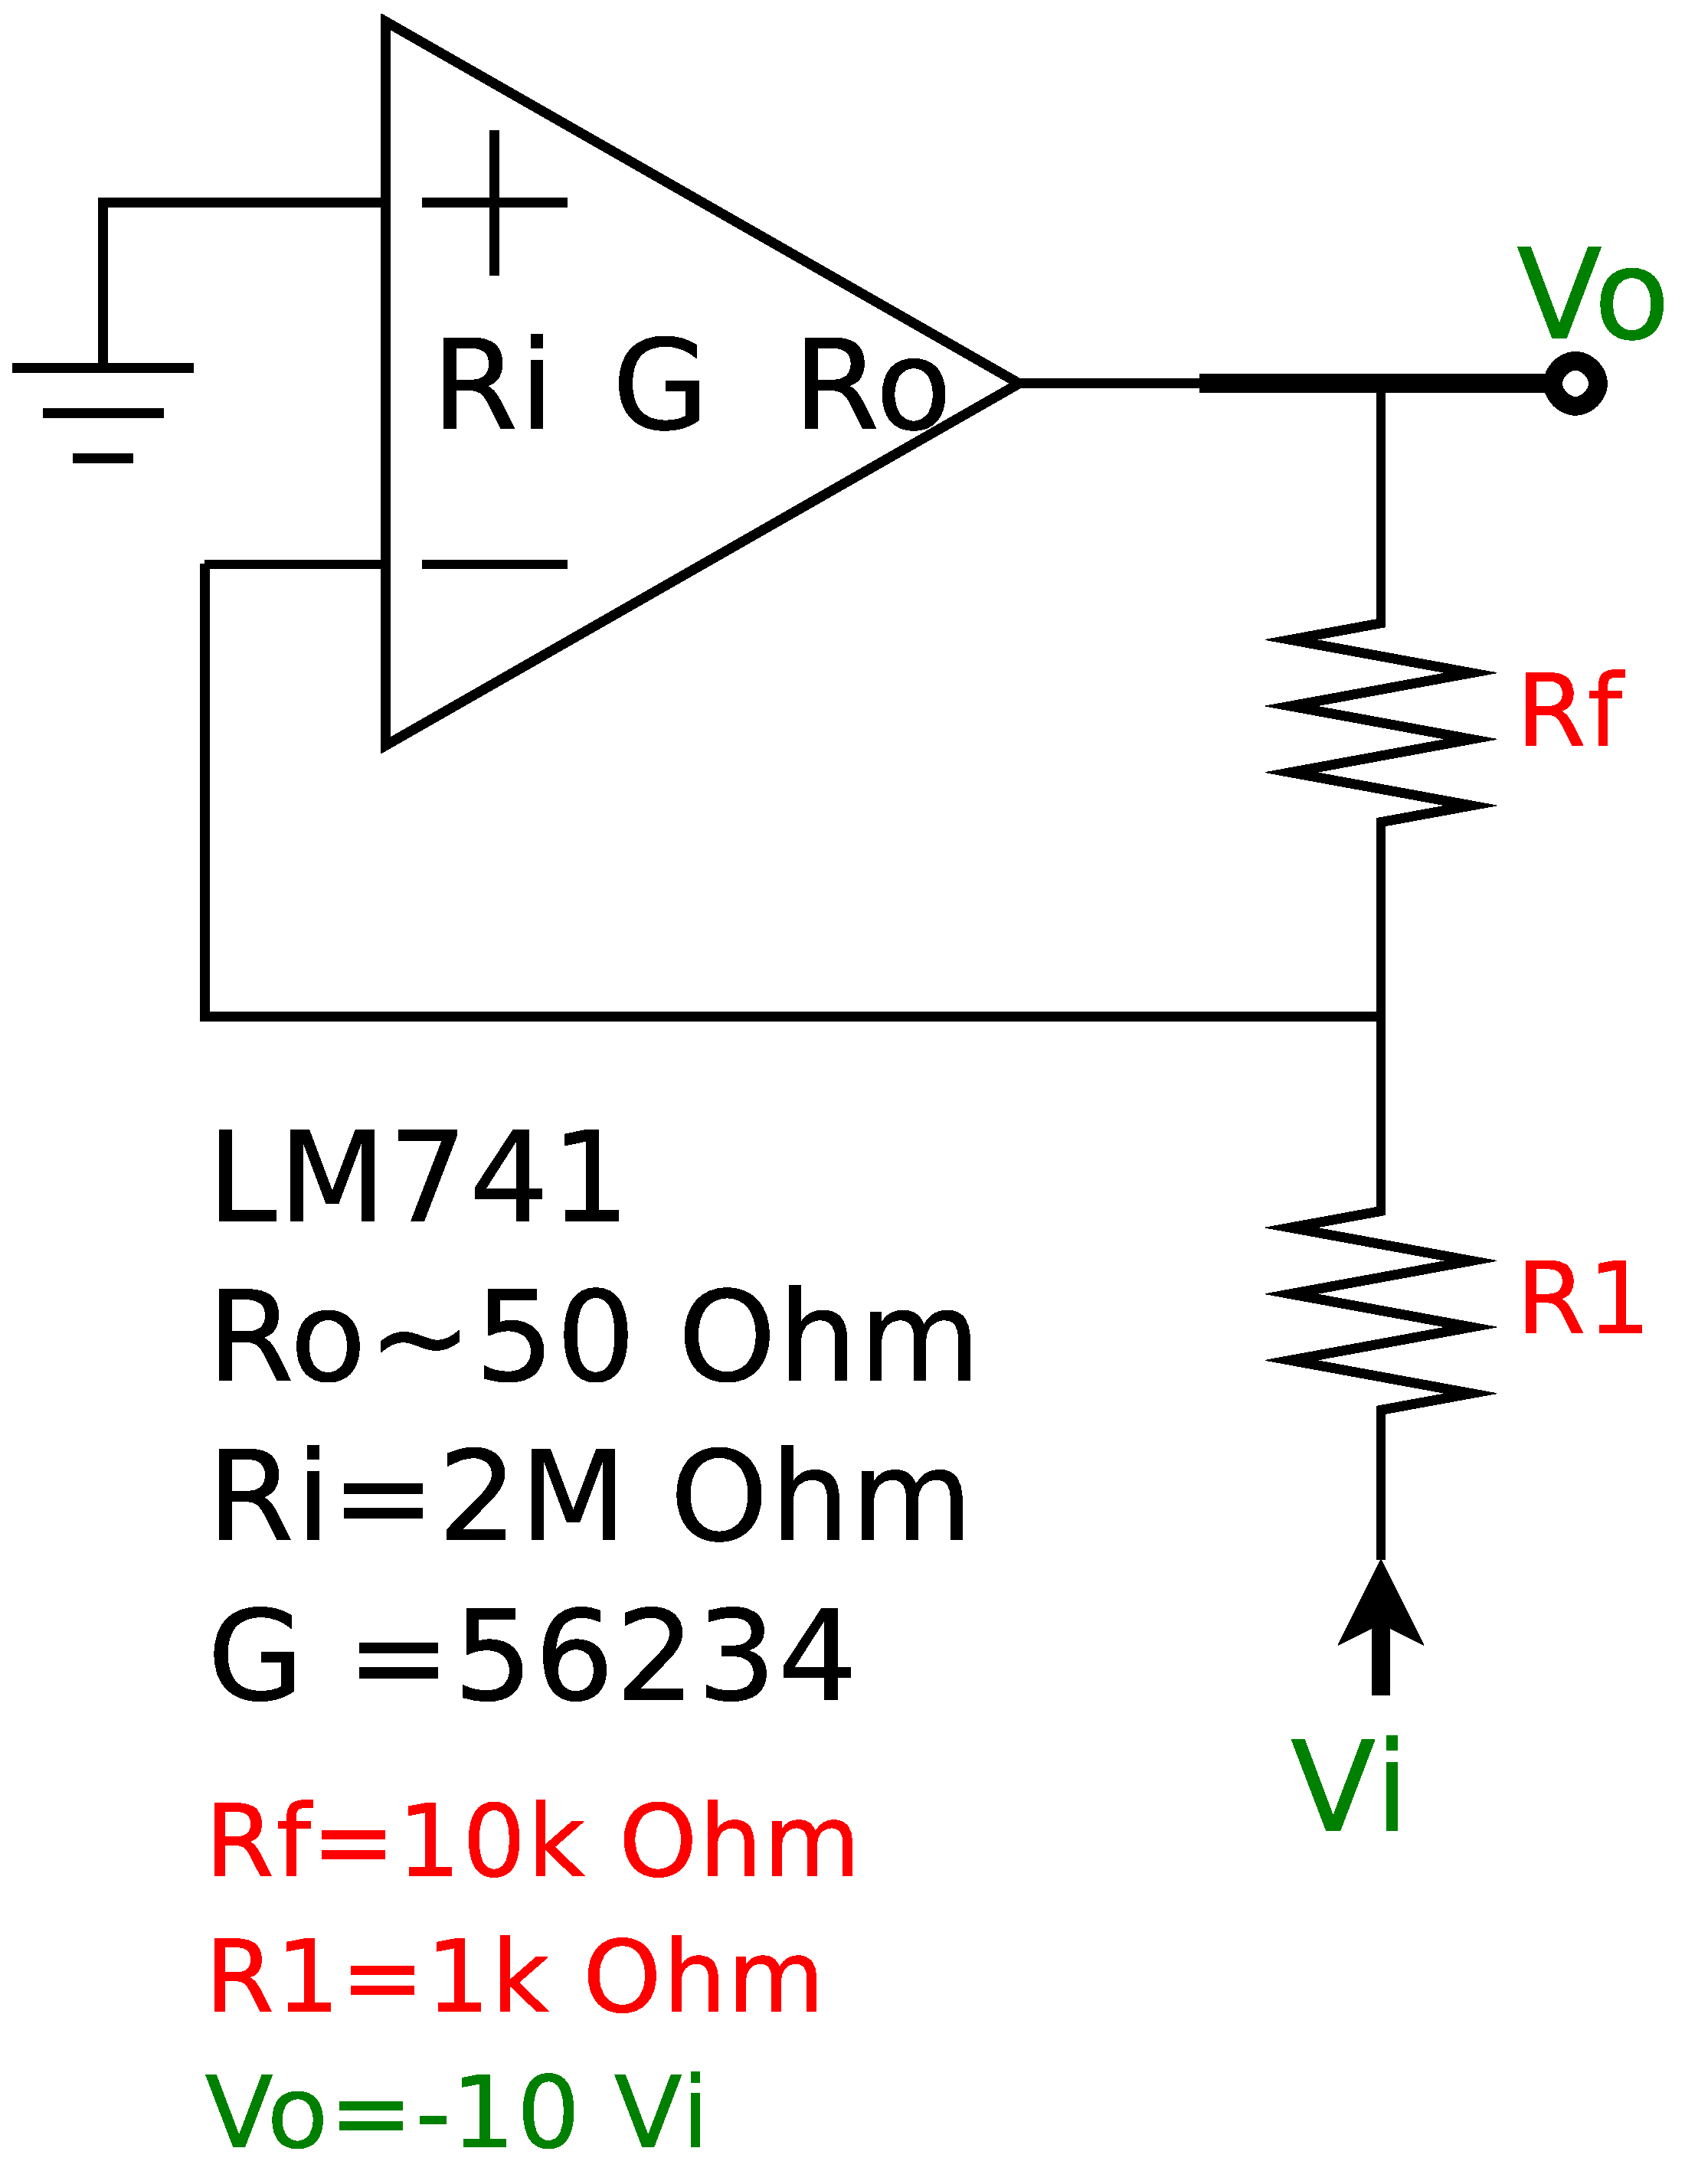
\includegraphics[width=0.9\textwidth]{images/Ejemplo1a.eps} 
\end{center} 
\end{minipage}%
\begin{minipage}[c]{0.6\textwidth}
\begin{description}
 \item[$R_o << R_f$] A resistência de saída do Opamp é muito menor à resistência ligada a ela. 
 \item[$R_i >> R_f, R_1$] A resistência de entrada do Opamp é muito maior as resistências envolvidas. 
 \item[$G >>\frac{ R_f }{ R_1}$] O ganho do Opamp deve ser maior ao valor absoluto do ganho do sistema.
\end{description} 
\end{minipage}
\end{frame}

%%%%%%%%%%%%%%%%%%%%%%%%%%%%%%%%%%%%%%%%%%%%%%%%%%%%%%%%%%%%%%%%%%%%%%%%%%%%%%%%
\begin{frame}{Amplificador não inversor}
\begin{minipage}[c]{0.4\textwidth}
\begin{center}
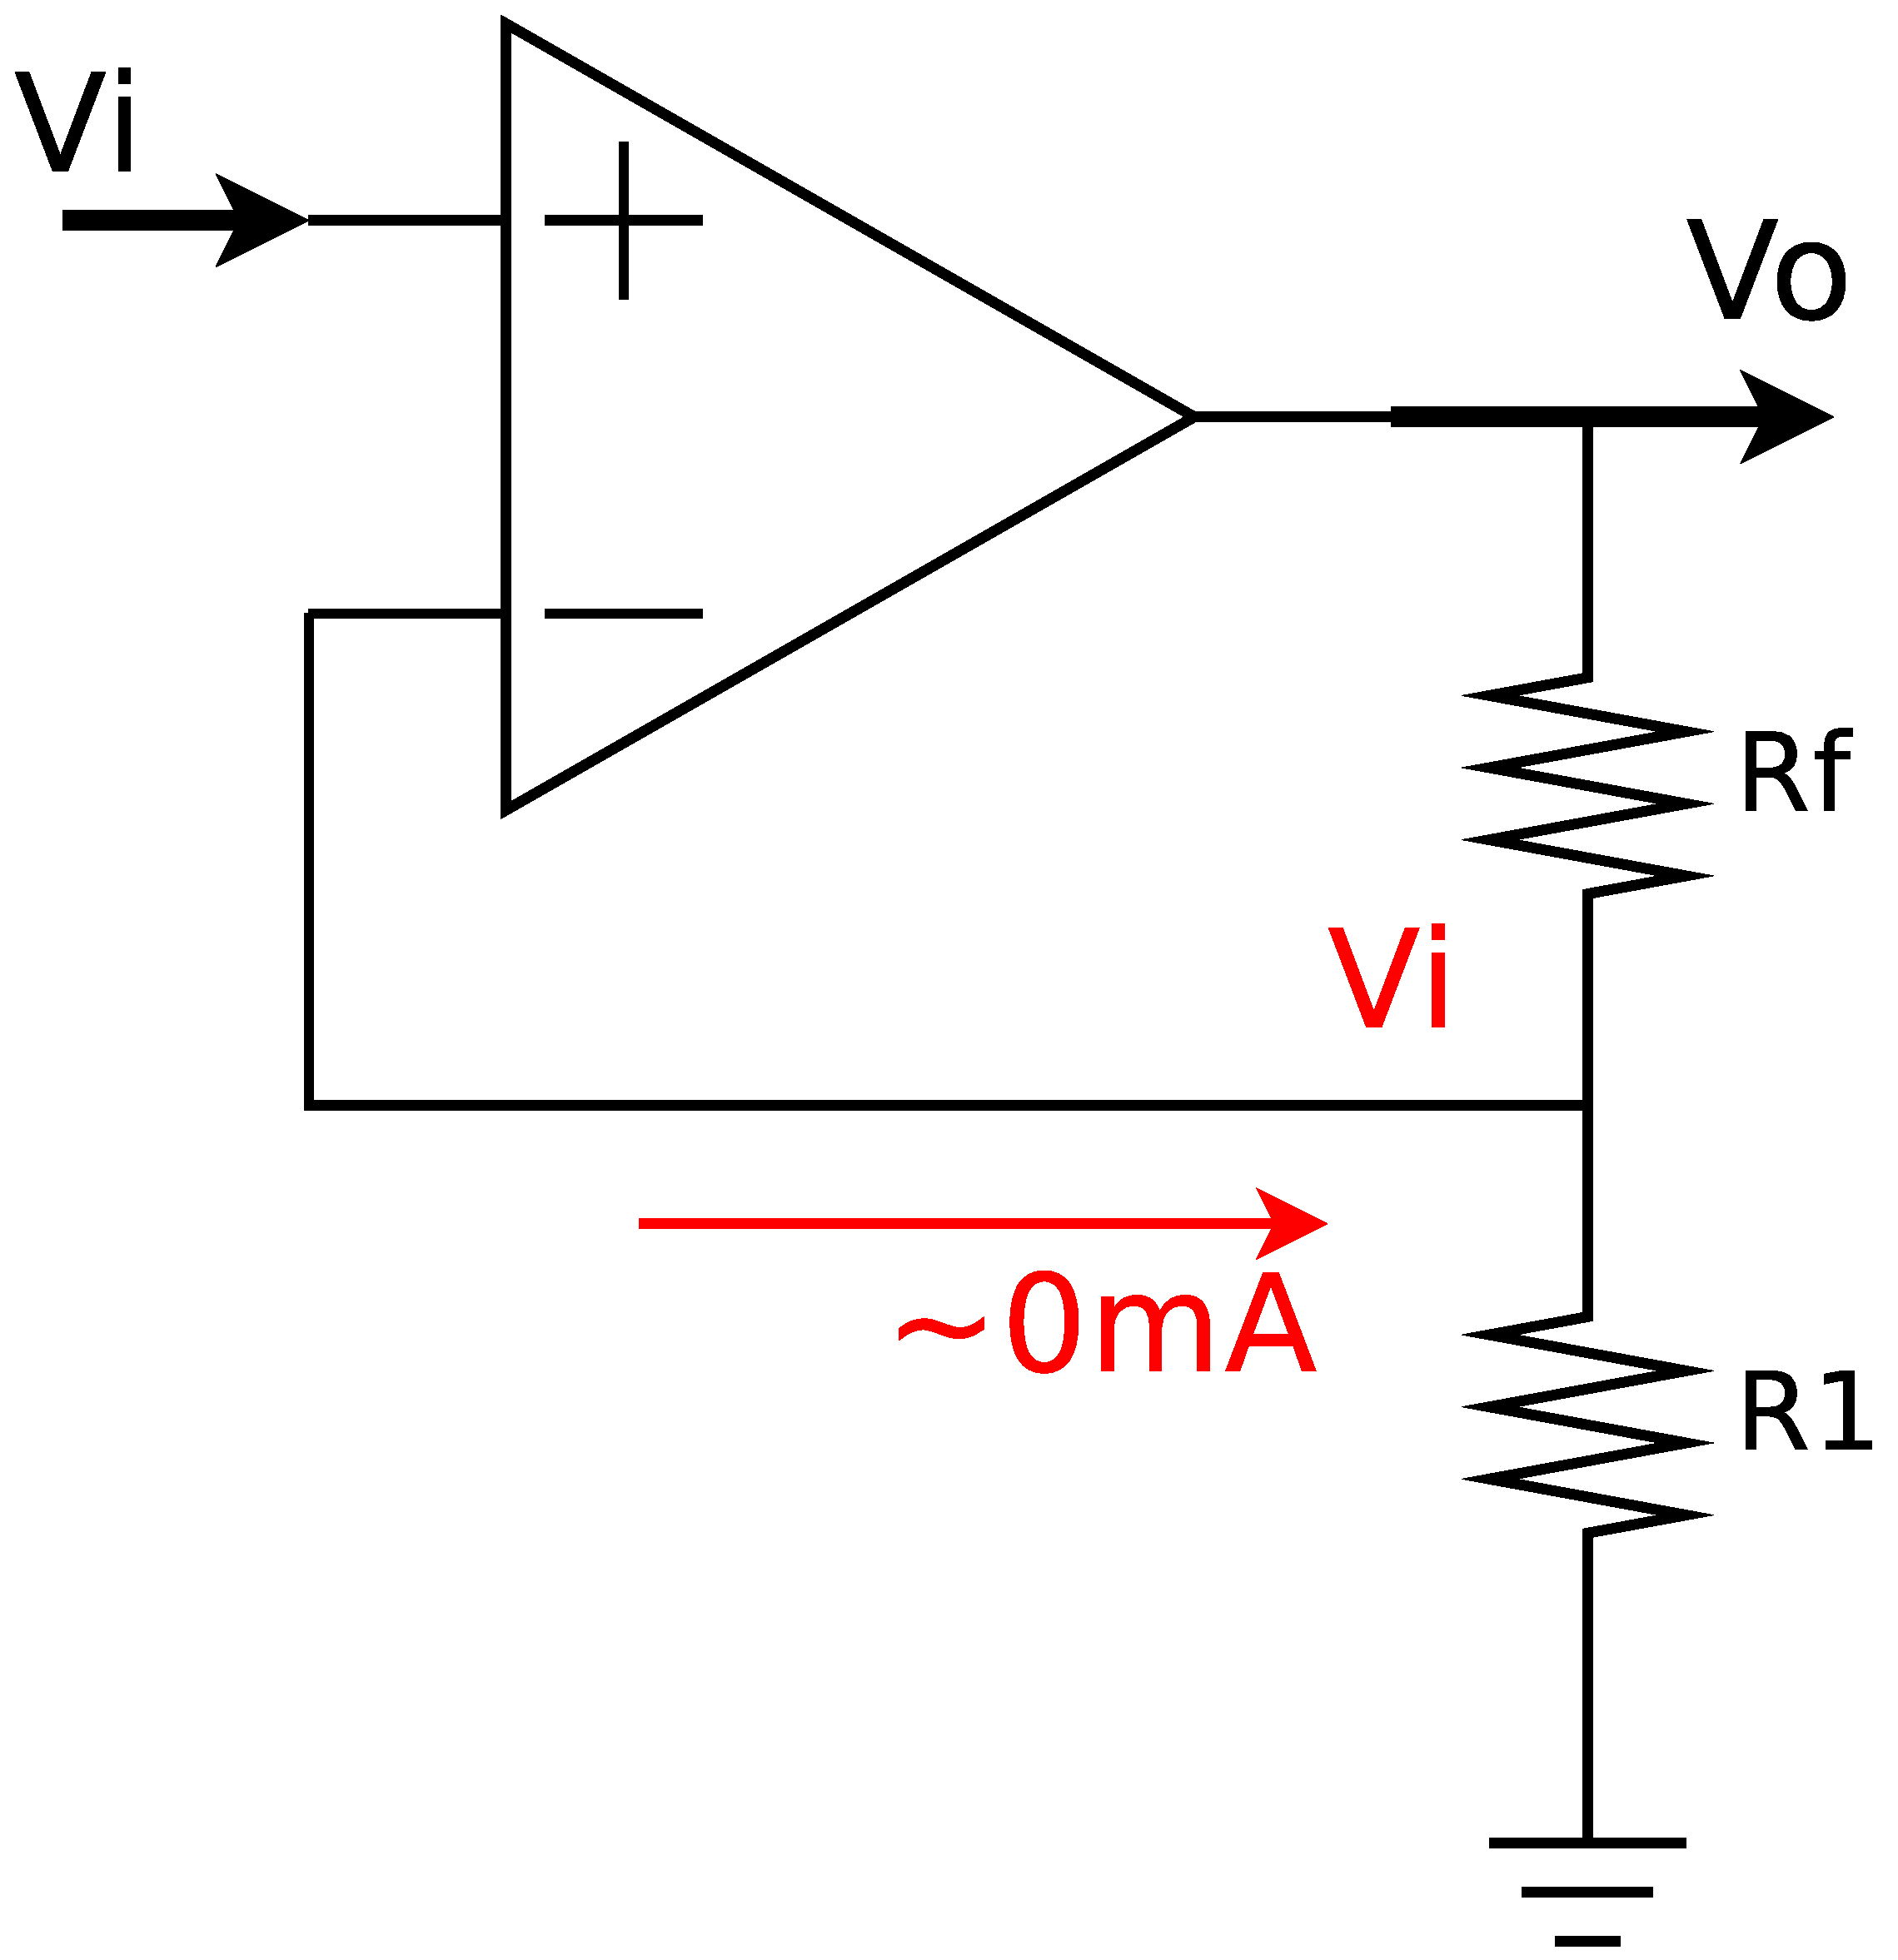
\includegraphics[width=0.9\textwidth]{images/Ejemplo2.eps} 
\end{center} 
\end{minipage}%
\begin{minipage}[c]{0.6\textwidth}
\begin{equation*}
 \frac{V_i}{R_1}=\frac{V_o}{R_1+R_f}
\end{equation*}
\begin{equation*}
 V_i \left( 1+\frac{R_f}{R_1} \right)=V_o
\end{equation*}
\end{minipage}
\end{frame}

% https://www.youtube.com/watch?v=gtzg43fhjYM
% http://www.curso-eletronica.com.br/artigos/realimentacao-positiva-e-negativa
% http://mit.ocw.universia.net/6-002/NR/rdonlyres/Electrical-Engineering-and-Computer-Science/6-002Circuits-and-ElectronicsFall2000/1A77B89E-22F7-4B74-B364-A292B8D4211B/0/6002L21.pdf
%%%%%%%%%%%%%%%%%%%%%%%%%%%%%%%%%%%%%%%%%%%%%%%%%%%%%%%%%%%%%%%%%%%%%%%%%%%%%%%%
\begin{frame}[allowframebreaks]
        \frametitle{References}
        \bibliographystyle{plain}
\bibliography{opamp}
\end{frame}



\end{document}
